\documentclass[journal,a4paper]{IEEEtran}
\usepackage[T1]{fontenc}
\usepackage[utf8]{inputenc}
\usepackage{graphicx}
\usepackage{booktabs}
\usepackage{array}
\usepackage{cite}
\usepackage{url}
\usepackage[hidelinks]{hyperref}
\usepackage{microtype}
\graphicspath{{figures/}}
\hypersetup{
  colorlinks=true, linkcolor=black, citecolor=black, urlcolor=blue,
  pdftitle={A Safe Harbour in a Cut-Throat World? General and Engineering-Specific Primal World Beliefs Among Indian Engineering Undergraduates},
  pdfauthor={Ritabrata Chakraborty},
  pdfsubject={Primal world beliefs, engineering education, measurement},
  pdfkeywords={primal world beliefs, PI-18, worldview, career security, acquiescent responding, reverse-keyed items, STEM higher education, India}}
\hyphenation{en-gi-neer-ing}

\begin{document}

\title{A Safe Harbour in a Cut-Throat World? General and Engineering-Specific Primal World Beliefs Among Indian Engineering Undergraduates}

\author{Ritabrata Chakraborty%
\thanks{R. Chakraborty is with the School of Engineering and Applied Science, University of Pennsylvania, Philadelphia, PA 19104 USA (e-mail: rcpenn28@engineering.upenn.edu). This research was conducted independently and received no funding.}}

\markboth{Primal World Beliefs Among Indian Engineering Undergraduates}{Chakraborty: A Safe Harbour in a Cut-Throat World?}

\maketitle

\begin{abstract}
Primal world beliefs (primals)—basic beliefs about whether the world is Safe, Enticing and Alive—predict well-being but have rarely been studied in non-Western students or alongside beliefs about a specific domain. A convenience sample of 108 Indian engineering undergraduates (aged 17–25) completed the 18-item Primals Inventory (PI-18) and 18 new, positively keyed engineering-specific items. Relative to published reference values, students saw the world as markedly less Safe ($d$ = $-$1.06), with the largest deviations on items describing the world as cut-throat and competitive (86.1\% agreed) and as bad. Yet they rated engineering as substantially safer than the world ($d_{\mathrm{z}}$ = 0.72, 95\% CI [0.51, 1.00]); this elevation persisted when only positively keyed general items were compared ($d_{\mathrm{z}}$ = 0.50) and was specific to Safe, with negligible differences for Enticing and Alive. General primals explained only 12\%–22\% of the variance in engineering-specific beliefs. Measurement analyses showed that reverse-keyed PI-18 items formed a method factor, and that the all-positive engineering items were dominated by one general factor and partly contaminated by acquiescence, except for the Safe subscale. Students may treat engineering as a protected pathway within a threatening world, consistent with compensatory-control and effort-justification accounts that require longitudinal testing. Domain-specific primal measures need balanced keying, and PI-18 studies in India should model keying effects. Data and code are available at \url{https://github.com/robotics1106/Primal-World-Beliefs-Engineering}.
\end{abstract}

\begin{IEEEkeywords}
PI-18, Worldview, Career Security, Acquiescent Responding, Reverse-Keyed Items, STEM Higher Education
\end{IEEEkeywords}

\section{Introduction}

Every engineering student in India arrives at university having passed through some version of the same filter: years of examination preparation, ranked entrance tests and admission processes in which a fraction of a mark can redirect a career~\cite{pienyu2024,subramanian2019}. Students who come through this process carry not only technical preparation but also beliefs about what kind of world they are living in—whether it rewards effort, whether others are allies or competitors, and whether the path they have chosen will keep them safe. Such beliefs are rarely measured in engineering education research, which has concentrated on skills, employability and mental health~\cite{blom2011,loyalka2021}.

Primal world beliefs, or \emph{primals}, offer a framework for measuring these beliefs. Primals are individuals' most basic beliefs about the overall character of the world, such as whether it is Safe, Enticing or Alive~\cite{clifton2019}. They are relatively stable, correlate substantially with depression, life satisfaction and flourishing~\cite{cliftonyaden2021}, and are only weakly related to objective circumstances such as wealth or neighbourhood safety~\cite{kerry2024}. They therefore appear to be lenses through which people interpret experience rather than summaries of it. A brief instrument, the PI-18~\cite{cliftonyaden2021}, has made primals easy to assess, but almost all published evidence comes from the United States, and a recent Indian validation could not reproduce the instrument's three-factor structure~\cite{bhatnagar2024}.

Two questions follow that existing research cannot answer. The first is descriptive and contextual: what do the primals of young people in a highly competitive, non-Western educational system look like? The second is theoretical: primals are defined as beliefs about the world \emph{as a whole}, but students also hold beliefs about the particular world of their discipline. Whether a student who sees the world as dangerous also sees engineering as dangerous—or instead sees engineering as a refuge from a dangerous world—is unknown. The answer matters for theory, because primals are assumed to colour perception across domains~\cite{clifton2019}, and for practice, because educators can influence beliefs about their programmes more readily than beliefs about the world.

This study addresses both questions in a sample of Indian engineering undergraduates who completed the PI-18 together with 18 newly written items that apply the Safe, Enticing and Alive primals to engineering education. Its contribution is principally empirical and methodological rather than a new theory. Empirically, it provides the first comparison of general and domain-specific primals within the same individuals and documents a selective ``safety premium'' for engineering: students rated engineering as markedly safer than the world, but no more enticing or purposeful. Methodologically, it shows how keying direction shapes primal measurement in this population, extending the Indian validation evidence~\cite{bhatnagar2024} and identifying design requirements for future domain-specific primal measures. Throughout, findings that follow from the data are distinguished from interpretations that remain to be tested.

\section{Literature Review}

\subsection{Primal World Beliefs and Their Measurement}

Clifton \emph{et al.}~\cite{clifton2019} identified 26 primals through a multi-method programme and organised them hierarchically. At the top is Good, the belief that the world is a good rather than a bad place. Beneath it are three secondary primals: Safe (the world is safe rather than dangerous), Enticing (the world is interesting and beautiful rather than dull) and Alive (the world is intentional and responsive rather than mechanistic). Tertiary primals include Cooperative, Regenerative and Harmless, each of which contributes to Safe. The PI-18 measures Safe with six items, Enticing with seven and Alive with five; Good is scored from 15 of the 18 items~\cite{cliftonyaden2021}. Seven items are reverse-keyed.

Three findings about primals frame the present study. First, primals are consequential: in large samples, PI-18 Good correlated $-$.49 with depression and .49 with life satisfaction~\cite{cliftonyaden2021}, and across 48 occupations more negative primals were associated with lower life satisfaction and flourishing and with no advantage in job success, even where threat vigilance might be expected to help~\cite{cliftonmeindl2022}. Second, primals are stable. Test–retest correlations over weeks approach .80~\cite{cliftonyaden2021}, and primals barely shifted during the onset of the COVID-19 pandemic~\cite{ludwig2023}. Third, primals are only loosely tied to circumstances. Across indicators of privilege, the average correlation with positive primals was $| r |$ = .09~\cite{kerry2024}, and associations with ad hoc experiences have generally been small~\cite{clifton2020}. In this respect, primals resemble the ``assumptive world'' that Janoff-Bulman~\cite{janoff1989} argued people use to make sense of events.

Evidence from outside the United States is scarce, a common problem in psychology~\cite{henrich2010}. Bhatnagar and Singh~\cite{bhatnagar2024} administered the PI-18 to English-speaking ($n$ = 266) and Hindi-speaking ($n$ = 272) Indian adults. The intended three-factor model did not fit either sample. An exploratory solution in the English sample produced a fourth factor that combined the reverse-keyed ``boring'', ``dull'' and ``getting worse'' items, and the authors ultimately recommended a nine-item unidimensional short form. Either the primal structure differs in India or item keying interferes with measurement there—a distinction the present study can examine.

\subsection{Generality Versus Domain Specificity}

Primals are, by definition, beliefs about the world in general. Yet much of educational psychology rests on the premise that beliefs relevant to learning are domain-specific. In situated expectancy–value theory, students' expectations of success and the value they assign to a task are tied to particular domains and contexts~\cite{eccles2020}. Interest develops through engagement with specific content~\cite{hidi2006}, and a sense of purpose for learning can be cultivated within a specific course of study~\cite{yeager2014}. It is therefore reasonable to ask whether domain analogues of the primals exist—for example, whether a student can believe that engineering is safe, enticing and purposeful—and how closely such beliefs track their general counterparts.

Two broad possibilities can be distinguished. Under a \emph{generalisation} account, primals act as top-down lenses~\cite{clifton2019}, so domain beliefs should closely mirror general beliefs in both level and rank order. Under a \emph{differentiation} account, domain beliefs are shaped by the particular institution, its incentives and its promises, and can diverge from general beliefs. One specific form of differentiation is compensatory. Compensatory control theory holds that when people perceive the world as random or threatening, they increase their investment in external systems that promise order and structure~\cite{kay2008,landau2015}. An engineering degree is, among other things, a highly structured system that promises a secure future. A complementary account comes from effort justification: people value outcomes more after investing heavily to obtain them~\cite{aronson1959}. The entrance-examination route to engineering in India requires exactly this kind of investment~\cite{subramanian2019}. Both accounts predict that engineering may be perceived as safer than the world, but neither predicts a comparable elevation for Enticing or Alive.

\subsection{Indian Engineering Education as a Context for Safe Beliefs}

India educates one of the world's largest engineering student populations, and the route into engineering is notably competitive. Subramanian~\cite{subramanian2019} describes how the national entrance examination system has made engineering a central symbol of merit and social mobility. Adolescents preparing for these examinations report high academic stress and parental pressure; in one recent Karnataka sample, 86\% of students reported high academic stress~\cite{pienyu2024}. Once enrolled, students face an uncertain labour market: employers have long reported gaps between graduates' skills and job requirements~\cite{blom2011}, and comparative assessments indicate that Indian engineering students make limited gains in critical thinking over the course of their degrees~\cite{loyalka2021}.

This context bears most directly on Safe, and particularly on its Cooperative facet. Social psychologists have long distinguished belief in a dangerous world from belief in a competitive jungle, in which life is a ruthless struggle for scarce resources~\cite{duckitt2002,perry2013}. The PI-18 item ``Instead of being cooperative, the world is a cut-throat and competitive place'' captures the latter. In an educational system organised around ranking, agreement with this statement may reflect an accurate description of students' experience rather than a generalised sense of threat, and the item may therefore behave differently as an indicator of Safe.

\subsection{Keying, Acquiescence and Cross-Cultural Measurement}

Mixing positively and negatively worded items is intended to reduce acquiescence, the tendency to agree regardless of content. However, reverse-keyed items often form their own method factor~\cite{marsh1996,weijters2013}, and these effects tend to be stronger outside Western, educated samples. Acquiescence varies systematically across cultures~\cite{smith2004}, and reverse-worded items have performed poorly in several Asian samples~\cite{wong2003}. Dialectical thinking—greater tolerance of apparent contradiction—offers a further, non-pejorative reason why some respondents agree with both a statement and its opposite~\cite{spencer2010}. For the present study, keying has two implications. It may distort the factor structure of the PI-18, as Bhatnagar and Singh's~\cite{bhatnagar2024} findings suggest, and it may inflate any instrument composed only of positively worded items. A domain-specific instrument with no reverse-keyed items could thus show apparent positivity that reflects response style rather than belief~\cite{podsakoff2003}.

\subsection{Research Questions}

The study addressed four research questions. Because no hypotheses were preregistered, the analyses are reported as tests of research questions, and analyses beyond these questions are labelled exploratory.

\textbf{RQ1 (measurement):} Do the PI-18 and the engineering-specific items show their intended three-dimensional structure in this sample, and how are they affected by item keying and acquiescence?

\textbf{RQ2 (general primals):} How do Indian engineering undergraduates' general primals compare with published reference values, and which beliefs differ most?

\textbf{RQ3 (domain versus general levels):} Do students rate engineering as more Safe, Enticing or Alive than the world in general, and is any difference specific to one primal?

\textbf{RQ4 (coupling):} How strongly are engineering-specific beliefs predicted by general primals, and does acquiescence contribute beyond them?

\section{Method}

\subsection{Design and Participants}

The study used a cross-sectional online survey and is reported following the STROBE guidelines for observational studies~\cite{vonelm2007}. The survey targeted undergraduate engineering students in India and was completed by a convenience sample between 13 and 15 October 2024. The analysis dataset comprises all 108 time-stamped responses recorded by the survey form. No responses had missing data, and no cases were excluded from the primary analyses; data-quality screening was used only for sensitivity analyses (see Data Quality). An earlier working tabulation of the data contained a further seven rows that could not be matched to time-stamped form submissions; these rows were not analysed.

Of the 108 respondents, 97 (89.8\%) were male and 11 (10.2\%) were female. Ages ranged from 17 to 25 years ($M$ = 18.86, $SD$ = 1.30, median = 19), and 90.7\% were aged 17–20, indicating a sample concentrated in the early years of undergraduate study. Respondents reported 20 different Indian states and union territories, grouped here into the north ($n$ = 50, 46.3\%), west ($n$ = 23, 21.3\%), south ($n$ = 22, 20.4\%), east ($n$ = 11, 10.2\%) and centre ($n$ = 2, 1.9\%); no respondent reported a north-eastern state. Year of study, engineering discipline and institution were not recorded.

\subsection{Measures}

\textit{General primals.} The PI-18~\cite{cliftonyaden2021} comprises 18 statements about the world, answered on a six-point scale from \emph{strongly disagree} to \emph{strongly agree}. Responses were scored 0–5 following the published key, with the seven reverse-keyed items rescored (5 $-$ $x$). Safe, Enticing and Alive scores are the means of their 6, 7 and 5 items, respectively, and Good is the mean of 15 items (all Safe and Enticing items plus two Alive items). In the survey form, the items were grouped by intended primal rather than presented in the validated fixed order, and the optional attention-check item was not included.

\textit{Engineering-specific primal beliefs.} Eighteen items were written for this study to apply each secondary primal to engineering education. These items are referred to here as the Engineering Primal Beliefs items (EPB-18). Six Safe items address the security of the engineering pathway (e.g., ``I trust that my education is preparing me for a stable career in engineering''), six Enticing items address the interest and possibility of engineering (e.g., ``The complexity of engineering makes it fascinating to study and work in'') and six Alive items address purpose and meaning (e.g., ``The work I do in engineering feels connected to something bigger than myself''). All items are positively keyed and used the same six-point response format. Full item wording is given in Supplementary Table~\ref{tab:s1} in the Supplementary Material at the end of this paper. Scores are item means on a 0–5 metric, so that 2.5 marks the boundary between net disagreement and net agreement.

\subsection{Procedure and Ethical Considerations}

Participants completed the survey anonymously through an online form that collected sex, age and state, followed by the PI-18 and EPB-18 items. No names, e-mail addresses, student identifiers or institutional affiliations were collected, and no participant can be identified from the data. In the shared dataset, state is recoded into broad regions and time stamps are removed to further reduce re-identification risk. The study was conducted independently by the author and was not reviewed by an institutional ethics committee. The form stated that participation was voluntary and anonymous, and submitting it was taken as consent; respondents aged 17 ($n$ = 10) took part under the same procedure, and no parental consent was sought.

\subsection{Data Quality}

Three indicators were computed. \emph{Long-string} responding was defined as the identical response to at least 18 consecutive items, half the item set~\cite{curran2016,meade2012}. \emph{Same-side responding} counted how many of eight antonym pairs within the PI-18 (e.g., ``I tend to see the world as pretty safe'' and ``On the whole, the world is a dangerous place'') a respondent answered on the same side of the scale. A \emph{content-balanced acquiescence index} was computed as the mean of two averages of raw, unreversed responses for the Safe and Enticing scales: the average of the positively keyed items and the average of the reverse-keyed items. Each of these subscales has three reverse-keyed items, so trait content approximately cancels while a general tendency to agree does not. The index is expressed on the original $-$5 to +5 response metric, where 0 indicates no net agreement. Alive was excluded from the index because it has only one reverse-keyed item.

\subsection{Analytic Strategy}

For RQ1, internal consistency was estimated with Cronbach's $\alpha$ (with 4,000-sample bootstrap CIs) and McDonald's $\omega$~\cite{mcneish2018}. The number of factors was assessed using Horn's~\cite{horn1965} parallel analysis (1,000 random data sets, 95th percentile criterion), followed by exploratory factor analysis (minimum residual, oblimin rotation). Confirmatory factor analyses (CFA) used maximum-likelihood estimation, which performs adequately with six or more response categories~\cite{rhemtulla2012}. For the PI-18, one-factor and three-factor models were compared with a three-factor model that added an orthogonal method factor on the seven reverse-keyed items~\cite{marsh1996}. For the EPB-18, one-, two- and three-factor models were compared. Fit was evaluated with $\chi ^2$, CFI, TLI, RMSEA and SRMR~\cite{hu1999}, interpreted comparatively given $N$ = 108. Discriminant validity was examined with latent correlations and the heterotrait–monotrait ratio (HTMT)~\cite{henseler2015}, and the strength of a general factor with Schmid–Leiman $\omega _{\mathrm{h}}$ and explained common variance (ECV)~\cite{rodriguez2016}.

For RQ2, scale means were compared with reference values computed from the item means of Clifton and Yaden's~\cite{cliftonyaden2021} Study 2 ($N$ = 5,171), using one-sample $t$ tests and standardised differences ($d$). Item-level tests were Holm-adjusted. Because measurement invariance across the two samples could not be tested, these comparisons are treated as descriptive benchmarks rather than estimates of cultural differences~\cite{milfont2010}.

For RQ3, paired $t$ tests compared engineering-specific and general scores for each primal, with $d_{\mathrm{z}}$ and bootstrap CIs~\cite{lakens2013} and Wilcoxon signed-rank tests as a robustness check. Because the EPB-18 items are all positively keyed whereas the PI-18 subscales mix keying, each comparison was repeated using only the positively keyed PI-18 items (the \emph{keying-matched} comparison). The specificity of any difference was tested by comparing the Safe gap (engineering minus general) with the Enticing and Alive gaps.

For RQ4, Pearson correlations with bootstrap CIs and disattenuated correlations were computed between general and engineering-specific scores. Hierarchical regressions predicted each engineering-specific score from the three general primals (Step 1) and then the acquiescence index (Step 2). Exploratory analyses examined associations with age and sex, Holm-adjusted across 16 tests. A sensitivity analysis repeated the key estimates after excluding long-string responders. Analyses were conducted in Python 3.13 using pandas, SciPy, statsmodels, factor\_analyzer 0.5.1 and semopy 2.3.11~\cite{igolkina2020}. Two-sided $\alpha$ = .05 was used throughout.

\section{Results}

\subsection{Data Quality}

Six respondents (5.6\%) gave identical answers to 18 consecutive items, in every case spanning the EPB-18 block: four answered every engineering item positively and two negatively. Same-side responding was common. Respondents answered a mean of 2.69 of the eight antonym pairs on the same side ($SD$ = 1.74), and 25.9\% placed ``the world is pretty safe'' and ``the world is dangerous'' on the same side of the scale. The content-balanced acquiescence index was positive on average ($M$ = 0.26 response-scale units, 95\% CI [0.09, 0.44], $t$(107) = 2.94, $p$ = .004, $d$ = 0.28), with 63.0\% of respondents above zero. The index was essentially uncorrelated with all general primals ($| r |$ $\le$ .07), supporting its interpretation as a content-free response style.

\subsection{RQ1: Measurement Structure}

\textit{PI-18.} Reliability was good for Enticing ($\alpha$ = .82), Alive ($\alpha$ = .85) and Good ($\alpha$ = .82) but modest for Safe ($\alpha$ = .68; Table~\ref{tab:t1}). Parallel analysis retained four factors (eigenvalues 4.90, 2.67, 1.75, 1.58). A three-factor exploratory solution recovered recognisable Enticing, Alive and Safe factors, but two reverse-keyed Safe items did not load on Safe: ``cut-throat and competitive'' had no loading above .23 on any factor, and ``things have a habit of getting worse'' loaded .38 on the Enticing factor and .10 on Safe (Supplementary Table~\ref{tab:s2}). In the three-factor CFA, these two items had the weakest standardised loadings (.14 and .29), and model fit was poor (Table~\ref{tab:t2}). Adding an orthogonal reverse-keying factor improved fit substantially, $\Delta \chi ^2$(7) = 77.22, $p$ < .001 (CFI = .877, RMSEA = .082, SRMR = .077). The method factor was defined most strongly by the reverse-keyed Enticing items (``boring'' .71, ``dull'' .62, ``not worth the effort'' .53). Composites of forward- and reverse-keyed items within the same primal correlated only moderately (Safe $r$ = .32, 95\% CI [.14, .48]; Enticing $r$ = .47 [.31, .61]). The latent correlations among primals resembled the published structure: Safe and Enticing correlated .50, Enticing and Alive .36, and Safe and Alive only .16.

\begin{table*}[tp]
\centering
\renewcommand{\arraystretch}{1.12}
\footnotesize
\caption{Descriptive Statistics and Reliability of General and Engineering-Specific Primal Belief Scales (N = 108)}
\label{tab:t1}
\begin{tabular}{>{\raggedright\arraybackslash}p{4.3cm}cccccccc}
\toprule
\textbf{Scale} & $k$ & $M$ [95\% CI] & $SD$ & $\alpha$ [95\% CI] & $\omega$ & \% > midpoint & Ref. $M$ & $d$ vs. ref. \\
\midrule
General Safe (PI-18) & 6 & 2.04 [1.89, 2.19] & 0.80 & .68 [.56, .76] & .67 & 22.2 & 2.88 & $-$1.06 \\
General Enticing (PI-18) & 7 & 3.33 [3.14, 3.52] & 1.00 & .82 [.76, .86] & .82 & 81.5 & 3.83 & $-$0.50 \\
General Alive (PI-18) & 5 & 2.71 [2.48, 2.95] & 1.24 & .85 [.79, .89] & .85 & 58.3 & 3.01 & $-$0.24 \\
General Good (PI-18) & 15 & 2.71 [2.57, 2.85] & 0.74 & .82 [.76, .86] & .81 & 62.0 & 3.35 & $-$0.86 \\
Engineering Safe (EPB-18) & 6 & 2.87 [2.66, 3.08] & 1.10 & .87 [.81, .91] & .87 & 64.8 & — & — \\
Engineering Enticing (EPB-18) & 6 & 3.54 [3.34, 3.73] & 1.02 & .87 [.81, .92] & .88 & 84.3 & — & — \\
Engineering Alive (EPB-18) & 6 & 2.96 [2.74, 3.18] & 1.13 & .89 [.85, .92] & .89 & 63.0 & — & — \\
Engineering total (EPB-18) & 18 & 3.12 [2.94, 3.30] & 0.95 & .94 [.91, .95] & .94 & 79.6 & — & — \\
\bottomrule
\end{tabular}

\vspace{2pt}\parbox{\textwidth}{\scriptsize \emph{Note.} All scores range 0–5 (higher = more Safe, Enticing, Alive or Good); reverse-keyed PI-18 items were rescored. $\alpha$ = Cronbach's alpha with 4,000-sample percentile bootstrap CI; $\omega$ = McDonald's omega total from a one-factor model. \% > midpoint = percentage of respondents scoring above 2.5, i.e., net agreement with the positive pole. Ref. M = mean of the item means reported for Study 2 ($N$ = 5,171) in the online supplement of Clifton and Yaden~\cite{cliftonyaden2021}; $d$ = (sample M $-$ Ref. M) / sample SD. All four differences from the reference values were significant, smallest $t$(107) = $-$2.45, $p$ = .016. No reference values exist for the engineering-specific items.}
\end{table*}

\textit{EPB-18.} The engineering-specific items were highly internally consistent (subscale $\alpha$ = .87–.89; total $\alpha$ = .94) but were dominated by a general factor. The first eigenvalue (8.71) accounted for 48.4\% of item variance and was 4.25 times the second (2.05); parallel analysis retained two factors, and the Schmid–Leiman solution gave $\omega _{\mathrm{h}}$ = .74 and ECV = .62. Mean inter-item correlations were .45 among engineering items, compared with .21 among PI-18 items and .15 between the two sets (Fig.~\ref{fig:f1}). The two-factor exploratory solution separated a Security factor (the six Safe items) from an Engagement–Meaning factor that combined the Enticing and Alive items. The three-factor CFA fitted better than the one- and two-factor models (Table~\ref{tab:t2}), but its fit remained marginal, and Enticing and Alive were not clearly distinct (latent $r$ = .79, HTMT = .86). By contrast, Engineering Safe was clearly distinct from Engineering Enticing (latent $r$ = .50, HTMT = .59). Item-level loadings (Supplementary Table~\ref{tab:s1}) located the overlap: the effort-and-perseverance item loaded weakly on Safe (.35), ``full of potential and discovery'' (intended Enticing) loaded on Alive (.70), and two Alive items cross-loaded on Enticing.

\begin{table*}[tp]
\centering
\renewcommand{\arraystretch}{1.12}
\footnotesize
\caption{Fit of Confirmatory Measurement Models for the General (PI-18) and Engineering-Specific (EPB-18) Items}
\label{tab:t2}
\begin{tabular}{>{\raggedright\arraybackslash}p{5.8cm}ccccc>{\raggedright\arraybackslash}p{5.0cm}}
\toprule
\textbf{Model} & $\chi ^2$ ($df$) & CFI & TLI & RMSEA & SRMR & Latent correlations / comparison \\
\midrule
\multicolumn{7}{l}{\emph{PI-18 (general primals)}} \\
\hspace{0.8em}One factor & 537.65 (135) & .444 & .370 & .167 & .145 &  \\
\hspace{0.8em}Three correlated factors (Safe, Enticing, Alive) & 291.34 (132) & .780 & .745 & .106 & .097 & $\varphi$: S–E = .50, S–A = .16, E–A = .36 \\
\hspace{0.8em}Three factors + orthogonal reverse-keying factor & 214.12 (125) & .877 & .849 & .082 & .077 & $\Delta \chi ^2$(7) = 77.22, p < .001 vs. three factors \\
\multicolumn{7}{l}{\emph{EPB-18 (engineering-specific)}} \\
\hspace{0.8em}One factor & 492.48 (135) & .711 & .673 & .157 & .102 &  \\
\hspace{0.8em}Two factors (Security; Engagement–Meaning) & 376.12 (134) & .804 & .777 & .130 & .092 & $\varphi$ = .67 \\
\hspace{0.8em}Three correlated factors (Safe, Enticing, Alive) & 316.37 (132) & .851 & .827 & .114 & .090 & $\varphi$: S–E = .50, S–A = .74, E–A = .79; $\Delta \chi ^2$(2) = 59.76 vs. two factors, $\Delta \chi ^2$(3) = 176.11 vs. one factor, both p < .001 \\
\bottomrule
\end{tabular}

\vspace{2pt}\parbox{\textwidth}{\scriptsize \emph{Note.} Maximum-likelihood estimation (semopy 2.3.11), $N$ = 108; all $\chi ^2$ tests $p$ < .001. $\varphi$ = standardised latent correlation; S = Safe, E = Enticing, A = Alive. The reverse-keying factor was specified on the seven reverse-keyed PI-18 items and constrained to be uncorrelated with the substantive factors. Conventional benchmarks (CFI/TLI $\ge$ .95, RMSEA $\le$ .06, SRMR $\le$ .08)~\cite{hu1999} are stringent for N $\approx$ 100 and 18 indicators, so fit is interpreted comparatively.}
\end{table*}

\begin{figure*}[tp]
\centering
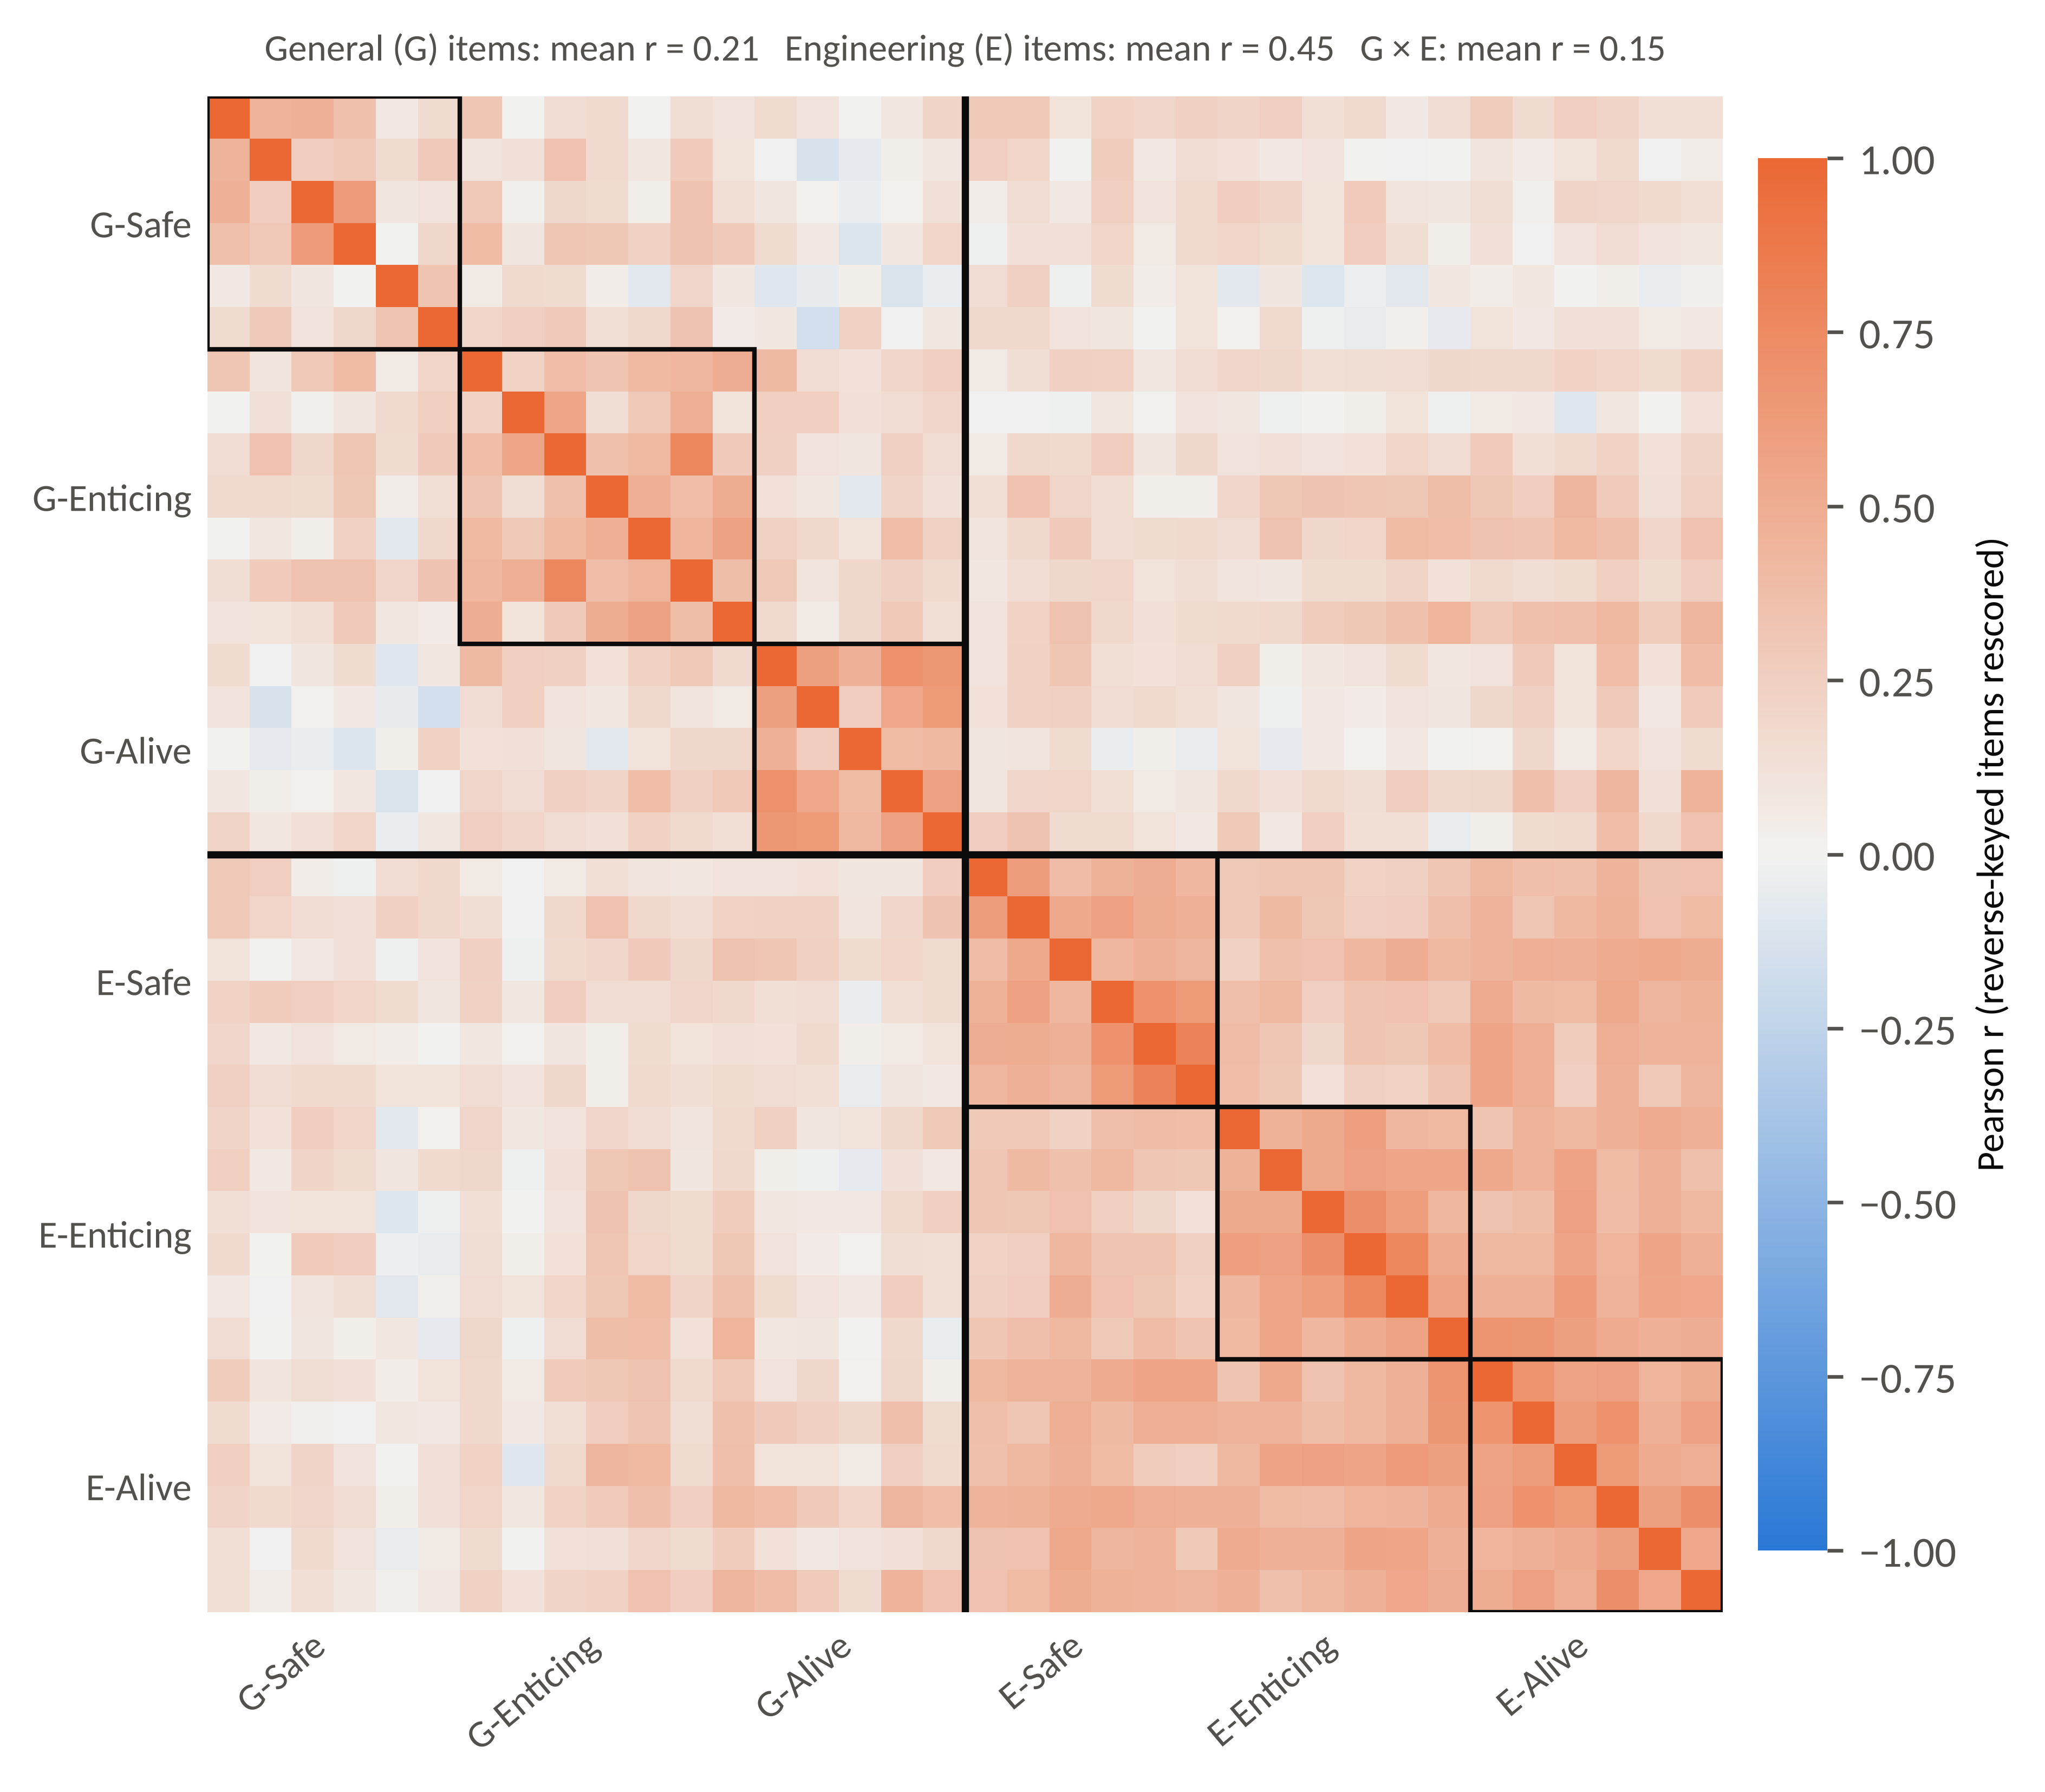
\includegraphics[width=0.55\textwidth]{fig3_item_correlations.png}
\caption{Item intercorrelations for the general (PI-18) and engineering-specific (EPB-18) items. Items are ordered by intended primal; reverse-keyed PI-18 items were rescored. Thin outlines mark intended subscales; thick lines separate the instruments ($N = 108$).}
\label{fig:f1}
\end{figure*}

\subsection{RQ2: General Primals Compared With Reference Values}

Students' general primals were below the reference values on every scale (Table~\ref{tab:t1}). The difference was largest for Safe ($M$ = 2.04 vs. 2.88; difference = $-$0.84, 95\% CI [$-$1.00, $-$0.69], $t$(107) = $-$10.96, $p$ < .001, $d$ = $-$1.06) and Good ($d$ = $-$0.86), moderate for Enticing ($d$ = $-$0.50) and small for Alive ($d$ = $-$0.24). Only 22.2\% of students scored above the midpoint on Safe, indicating that most leaned towards seeing the world as more dangerous than safe. At the item level (Fig.~\ref{fig:f2}; Supplementary Table~\ref{tab:s2}), the largest differences were for ``most things in the world are good'' ($d$ = $-$0.92), ``cut-throat and competitive'' ($d$ = $-$0.90) and ``things have a habit of getting worse'' ($d$ = $-$0.82). In absolute terms, 86.1\% of students agreed that the world is ``a cut-throat and competitive place'', 68.5\% that it is dangerous and only 31.5\% that it is ``pretty safe''. The two most explicitly teleological Alive items (``everything happens for a reason'', ``what happens \ldots{} is meant to happen'') did not differ from the reference values ($d$ = 0.06 and $-$0.04).

\begin{figure*}[tp]
\centering
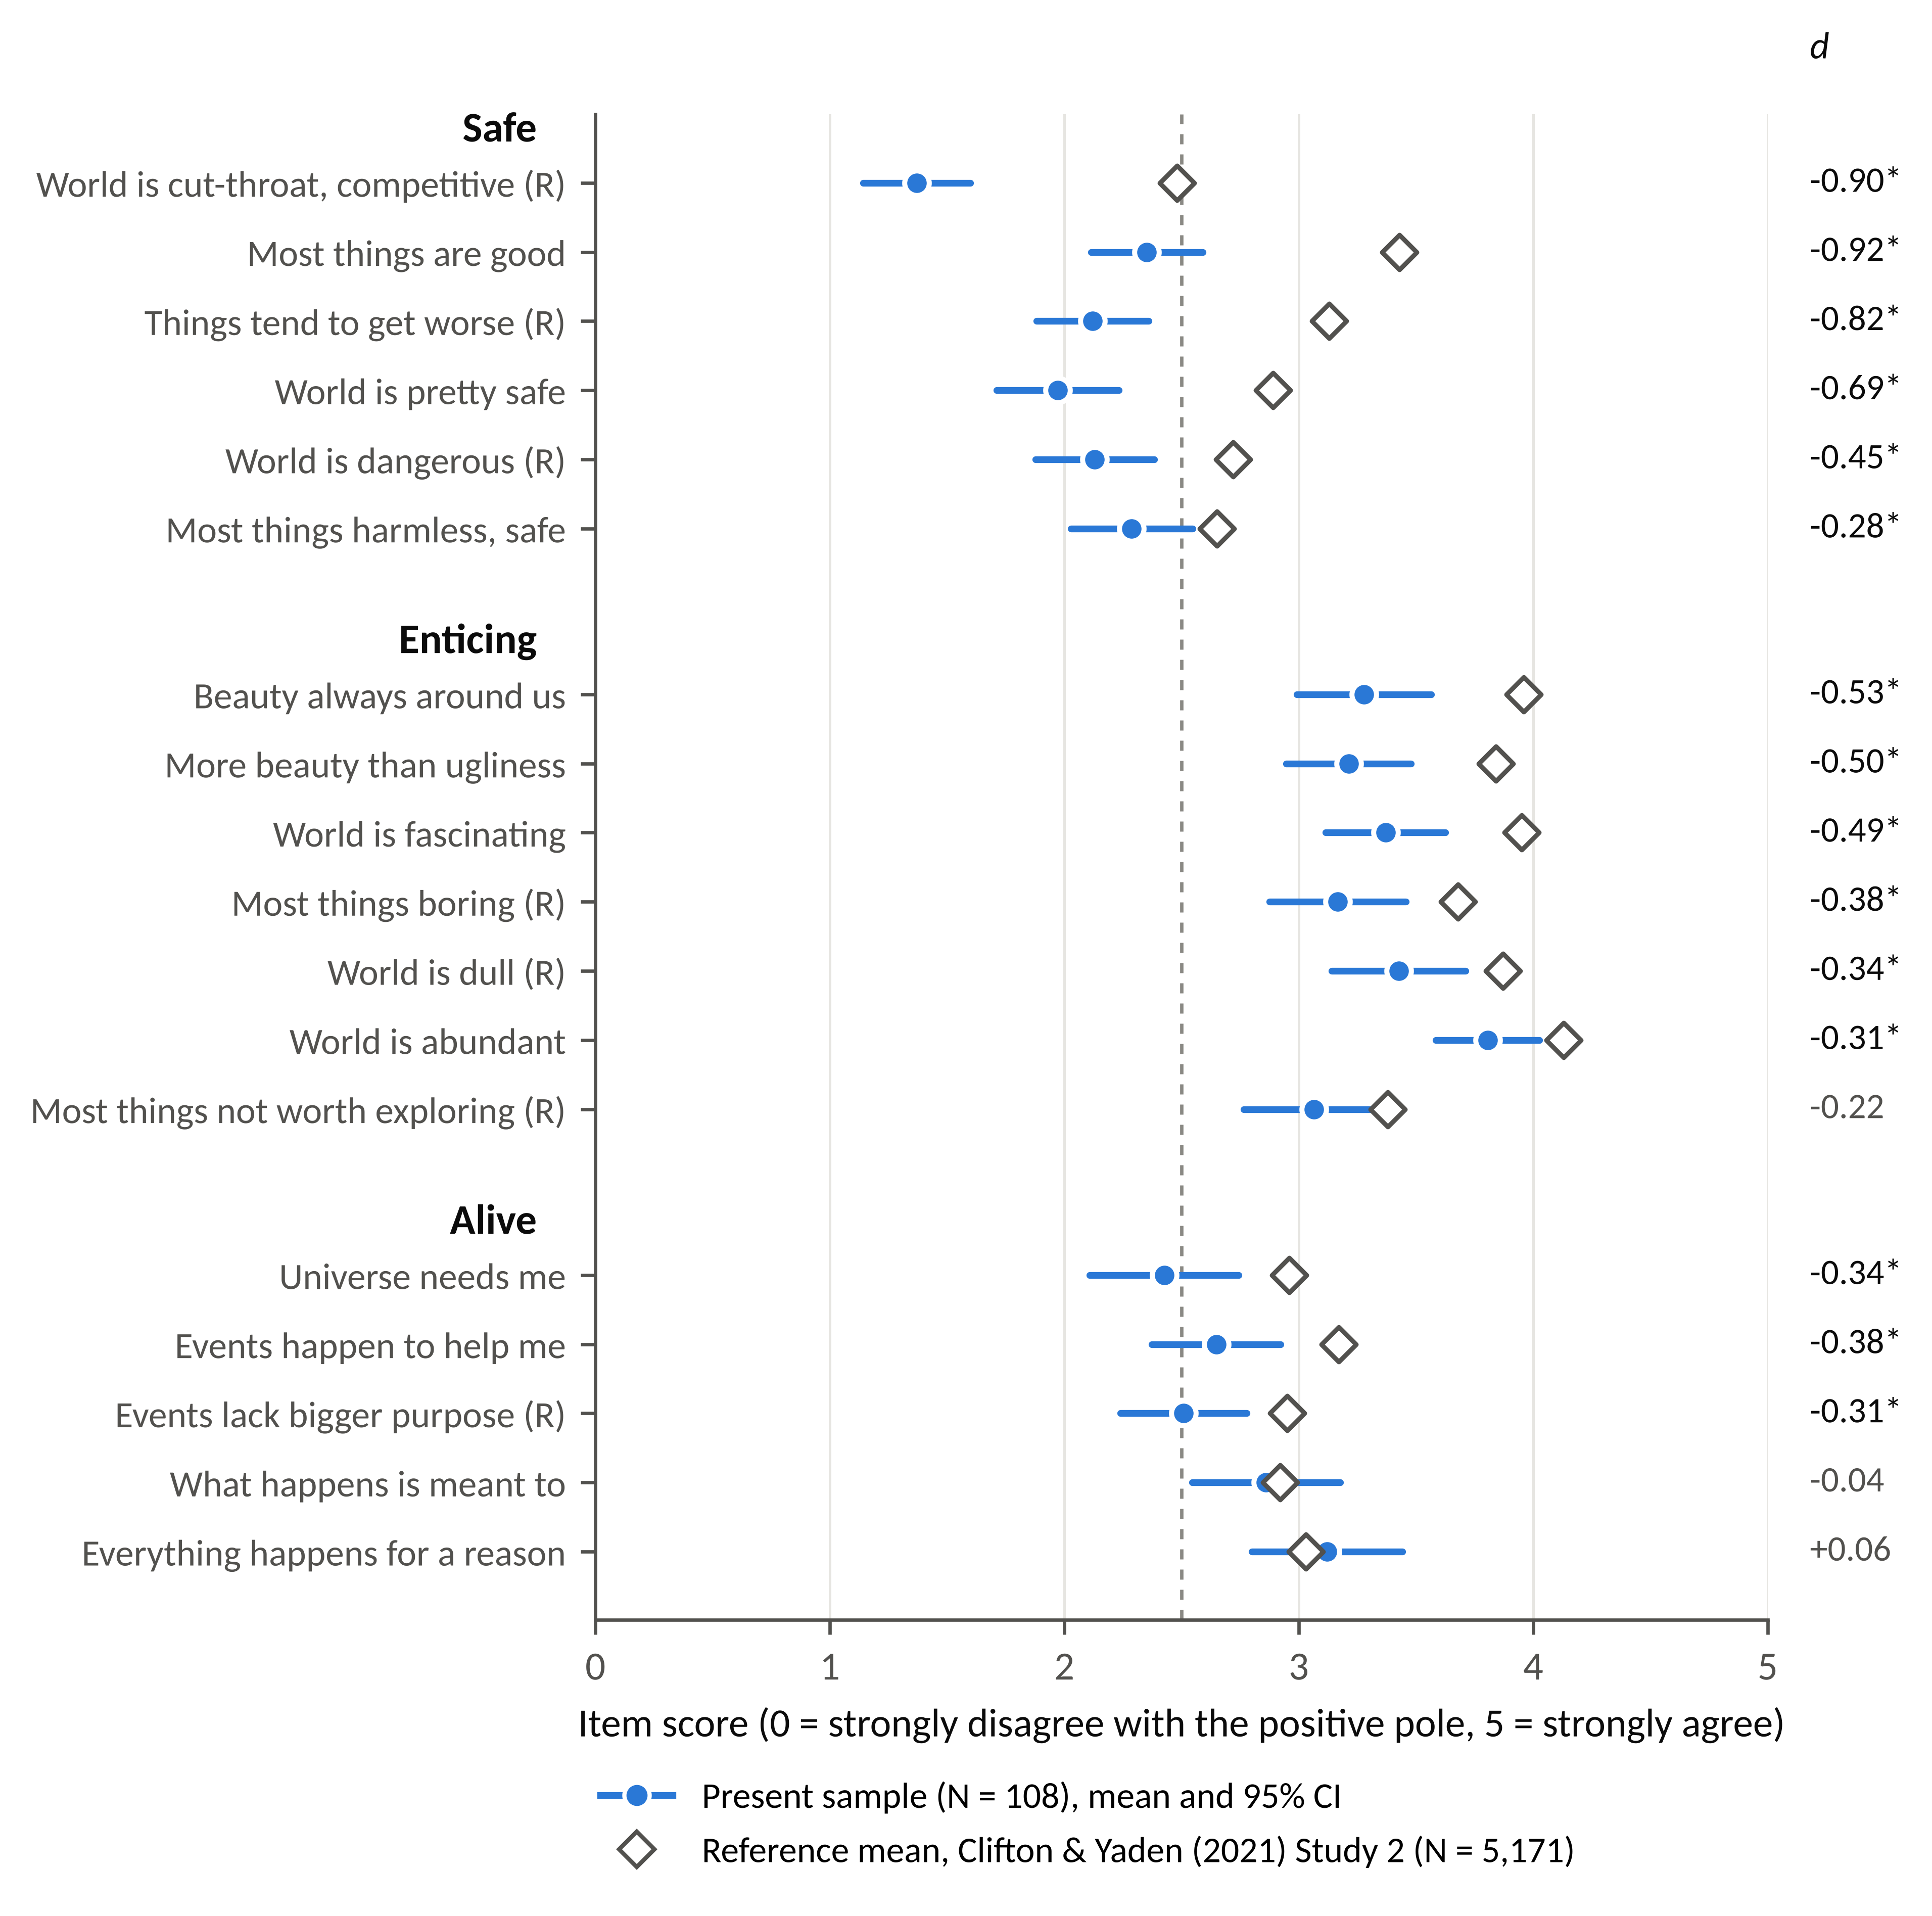
\includegraphics[width=0.7\textwidth]{fig1_items_vs_reference.png}
\caption{General primal items in the present sample (circles, means with 95\% CIs, $N = 108$) compared with published reference means (diamonds; Study~2 of \cite{cliftonyaden2021}, $N = 5{,}171$). Items marked (R) are reverse-keyed and shown after rescoring, so higher values indicate the positive pole. $d$ = standardised difference (pooled $SD$); * Holm-adjusted $p < .05$. Dashed line: scale midpoint.}
\label{fig:f2}
\end{figure*}

\subsection{RQ3: Engineering-Specific Versus General Beliefs}

Students rated engineering as considerably safer than the world (Table~\ref{tab:t3}; Fig.~\ref{fig:f3}A). Engineering Safe ($M$ = 2.87) exceeded general Safe ($M$ = 2.04) by 0.83 points (95\% CI [0.61, 1.05]), $t$(107) = 7.53, $p$ < .001, $d_{\mathrm{z}}$ = 0.72 [0.51, 1.00], and 79.6\% of students scored higher on engineering Safe than on general Safe. The difference was smaller but remained substantial in the keying-matched comparison, which used only the positively keyed general Safe items (difference = 0.67 [0.41, 0.92], $d_{\mathrm{z}}$ = 0.50, $p$ < .001). It therefore cannot be explained by the reverse-keyed items alone.

The elevation was specific to Safe. Engineering Enticing exceeded general Enticing by only 0.21 (95\% CI [$-$0.02, 0.43], $p$ = .07, $d_{\mathrm{z}}$ = 0.18), and engineering Alive exceeded general Alive by 0.25 ([$-$0.01, 0.51], $p$ = .06, $d_{\mathrm{z}}$ = 0.18). In keying-matched comparisons, neither difference approached significance ($d_{\mathrm{z}}$ = 0.11 and 0.14). The Safe gap was significantly larger than the Enticing gap (difference = 0.63 [0.38, 0.88], $t$(107) = 4.94, $p$ < .001, $d_{\mathrm{z}}$ = 0.48) and the Alive gap (0.59 [0.30, 0.88], $t$(107) = 3.99, $p$ < .001, $d_{\mathrm{z}}$ = 0.38). Both comparisons remained significant when keying-matched ($d_{\mathrm{z}}$ = 0.36 and 0.28, $p$ $\le$ .005).

At the person level (Fig.~\ref{fig:f3}B), 44 students (40.7\%) scored below the midpoint on general Safe but above it on engineering Safe. Of the 71 students who leaned towards seeing the world as dangerous, 44 (62.0\%) nonetheless saw engineering as safe. The reverse pattern—seeing the world as safe but engineering as unsafe—was rare ($n$ = 7, 6.5\%).

\begin{table*}[tp]
\centering
\renewcommand{\arraystretch}{1.12}
\scriptsize\setlength{\tabcolsep}{2.5pt}
\caption{Engineering-Specific Versus General Primal Beliefs: Within-Person Comparisons (N = 108)}
\label{tab:t3}
\begin{tabular}{>{\raggedright\arraybackslash}p{1.3cm}cccccccc}
\toprule
\textbf{Primal} & General $M$ ($SD$) & Engineering $M$ ($SD$) & Difference [95\% CI] & $t$(107) & $p$ & $d_{\mathrm{z}}$ [95\% CI] & Keying-matched difference [95\% CI] & Keying-matched $d_{\mathrm{z}}$ \\
\midrule
Safe & 2.04 (0.80) & 2.87 (1.10) & 0.83 [0.61, 1.05] & 7.53 & < .001 & 0.72 [0.51, 1.00] & 0.67 [0.41, 0.92] & 0.50 \\
Enticing & 3.33 (1.00) & 3.54 (1.02) & 0.21 [$-$0.02, 0.43] & 1.84 & .07 & 0.18 [$-$0.01, 0.38] & 0.12 [$-$0.09, 0.33] & 0.11 \\
Alive & 2.71 (1.24) & 2.96 (1.13) & 0.25 [$-$0.01, 0.51] & 1.89 & .06 & 0.18 [$-$0.01, 0.39] & 0.20 [$-$0.08, 0.47] & 0.14 \\
\bottomrule
\end{tabular}

\vspace{2pt}\parbox{\textwidth}{\scriptsize \emph{Note.} Paired-samples t tests; $d_{\mathrm{z}}$ = mean difference / SD of differences, with 5,000-sample percentile bootstrap CI. Wilcoxon signed-rank tests gave the same pattern (Safe $p$ < .001; Enticing $p$ = .033; Alive $p$ = .029). Percentage of students scoring higher on the engineering scale: Safe 79.6, Enticing 59.3, Alive 59.3. Keying-matched comparisons use only the positively keyed PI-18 items of each primal (Safe: 3 items; Enticing: 4; Alive: 4), because all EPB-18 items are positively keyed. The Safe gap exceeded the Enticing gap by 0.63 [0.38, 0.88], $d_{\mathrm{z}}$ = 0.48, and the Alive gap by 0.59 [0.30, 0.88], $d_{\mathrm{z}}$ = 0.38, both $p$ < .001.}
\end{table*}

\begin{figure*}[tp]
\centering
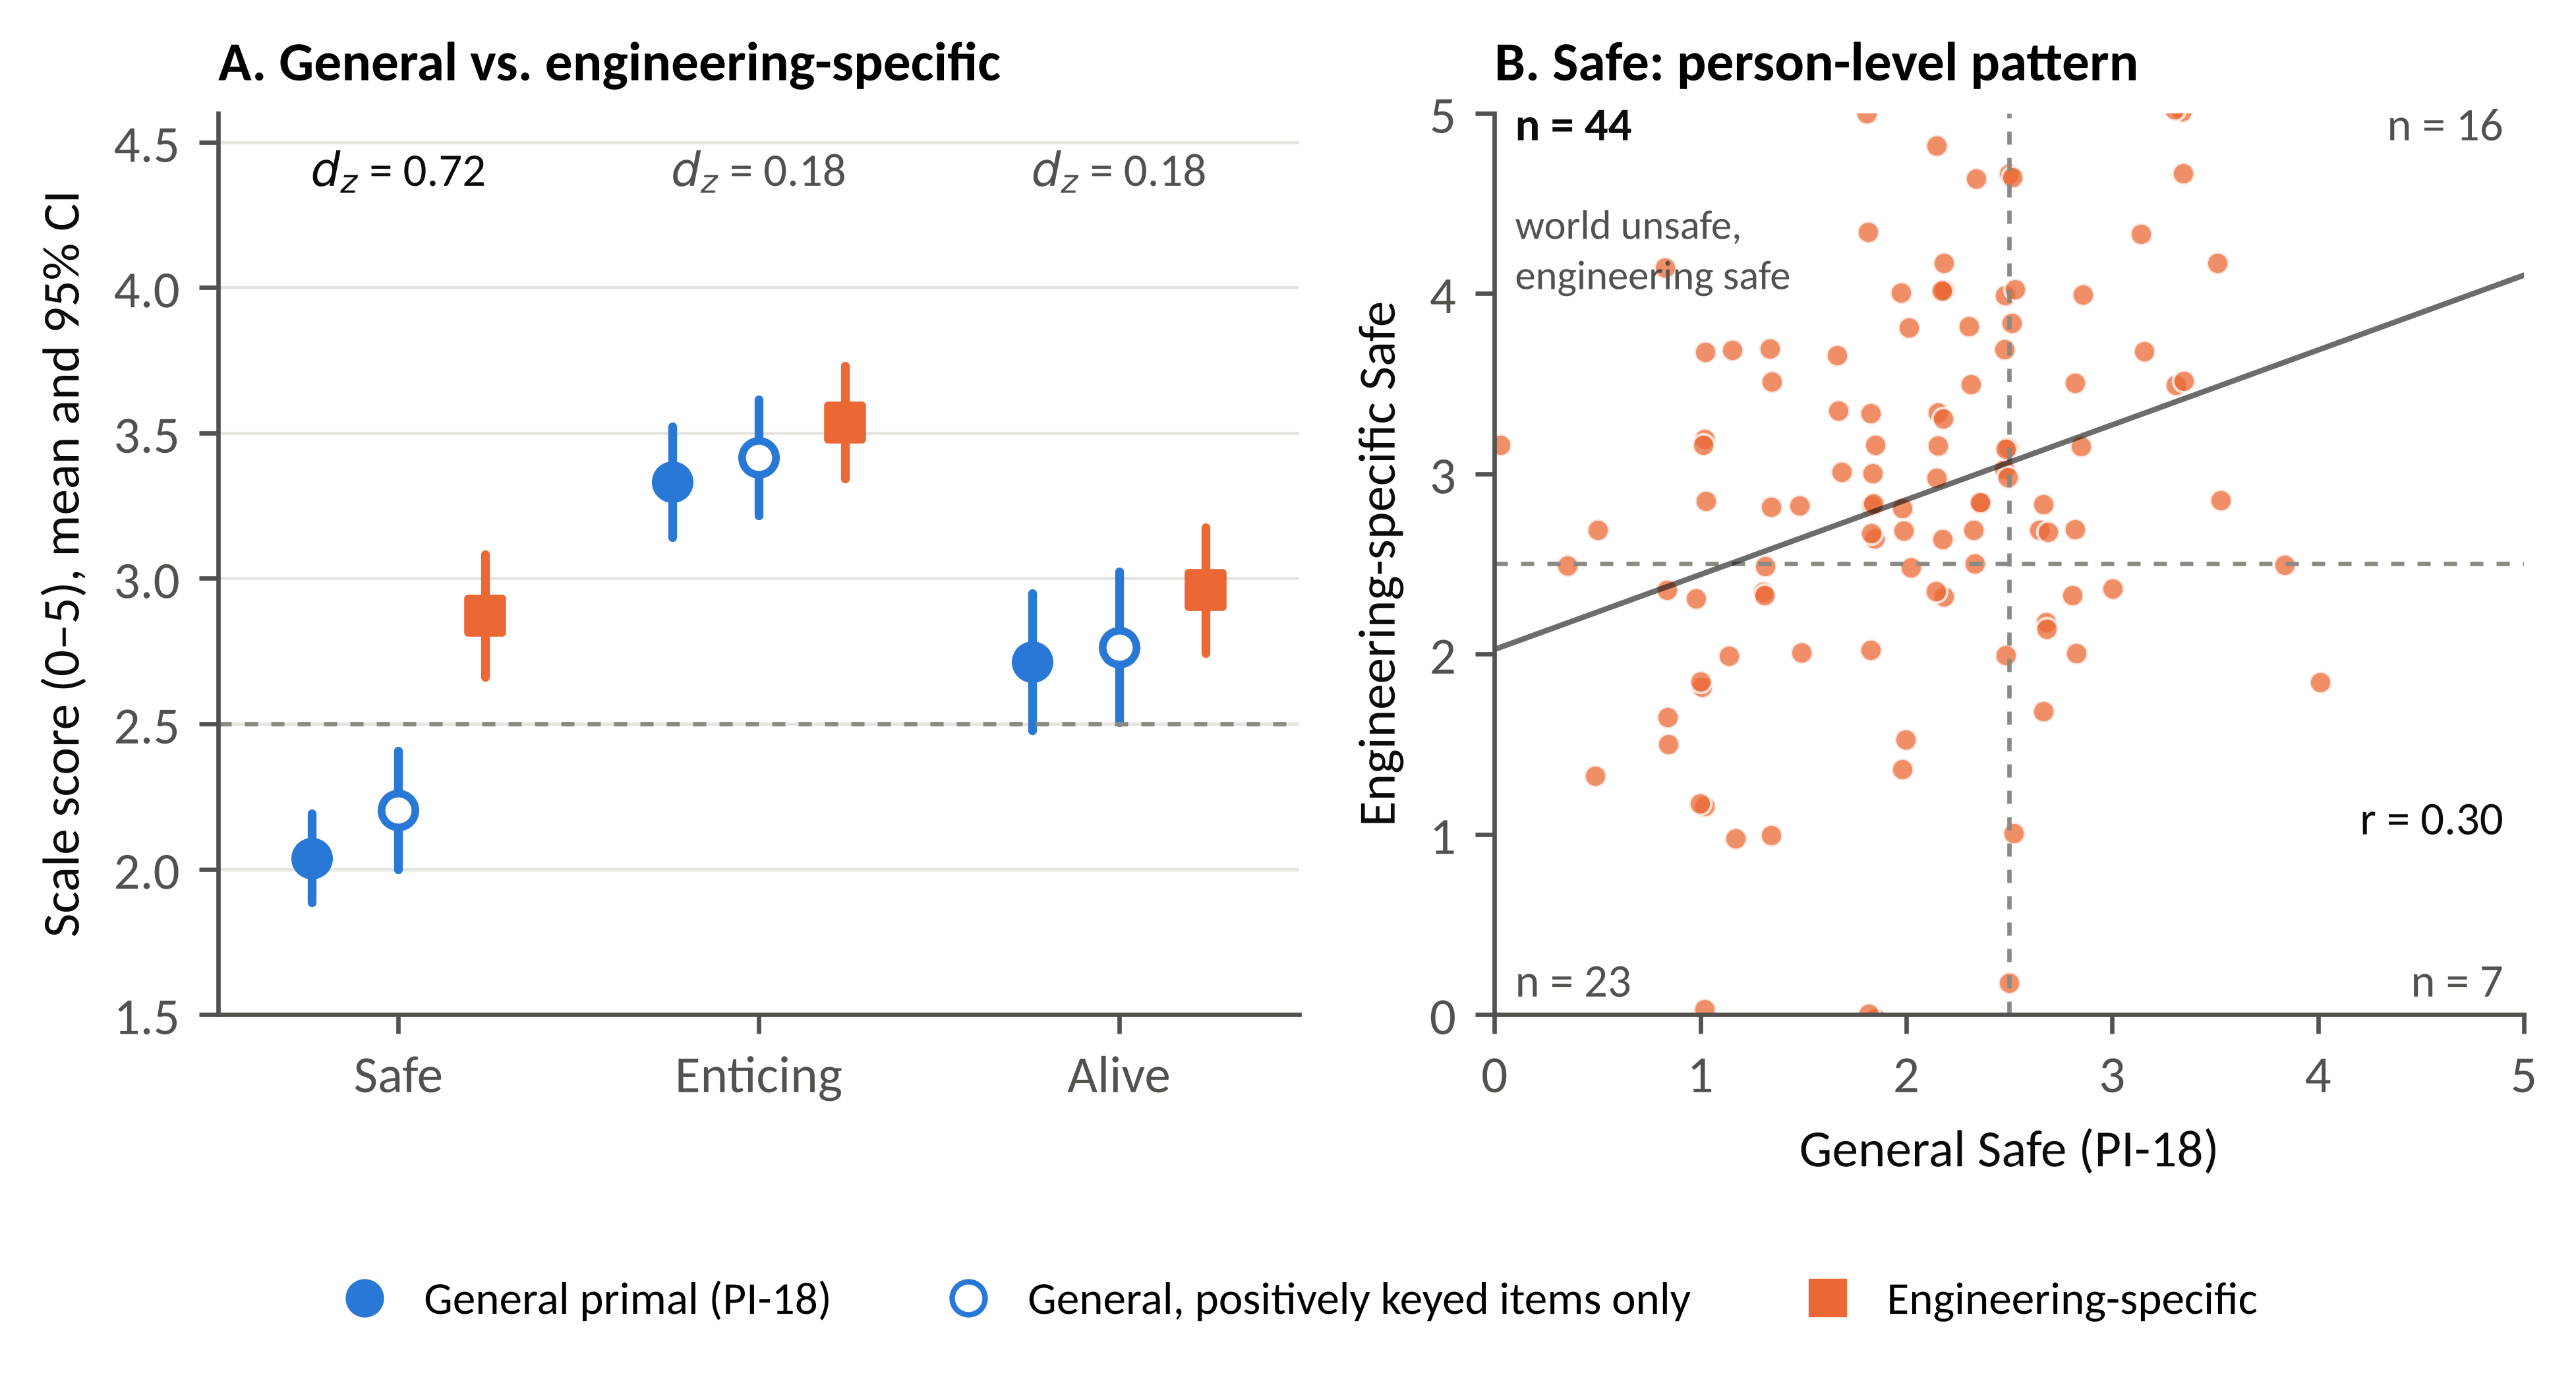
\includegraphics[width=0.9\textwidth]{fig2_domain_vs_general.png}
\caption{Engineering-specific versus general beliefs. (A) Means with 95\% CIs; hollow markers use only positively keyed PI-18 items (keying-matched comparison); $d_z$ refers to full-scale paired comparisons. (B) Each point is one student (jittered); dashed lines mark the midpoint; the solid line is the least-squares fit. Quadrant counts exclude 18 students exactly at the midpoint on either scale.}
\label{fig:f3}
\end{figure*}

\subsection{RQ4: Coupling With General Primals and Acquiescence}

General and engineering-specific beliefs were positively but only modestly related (Table~\ref{tab:t4}). Matched correlations were $r$ = .30 for Safe, .34 for Enticing and .35 for Alive (disattenuated $r$ $\approx$ .40 in each case). Coupling was not strictly primal-specific: general Enticing correlated more strongly with engineering Alive ($r$ = .40) than with engineering Enticing ($r$ = .34). Together, the three general primals explained 14\% of the variance in engineering Safe, 12\% in engineering Enticing, 22\% in engineering Alive and 19\% in the engineering total (Table~\ref{tab:t5}). The only unique general predictor of engineering Safe was general Safe ($\beta$ = .25, $p$ = .014).

Acquiescence affected the engineering subscales unequally (Fig.~\ref{fig:f4}; Table~\ref{tab:t5}). The acquiescence index correlated .27 (95\% CI [.09, .44]) with engineering Enticing and .19 [.01, .37] with engineering Alive, and it added significantly to their prediction beyond general primals ($\Delta R ^2$ = .083, $p$ = .001, and $\Delta R ^2$ = .040, $p$ = .02, respectively). It was unrelated to engineering Safe ($r$ = .07; $\Delta R ^2$ = .004, $p$ = .51).

\begin{table*}[tp]
\centering
\renewcommand{\arraystretch}{1.12}
\footnotesize
\caption{Pearson Correlations Among General and Engineering-Specific Primal Beliefs, Acquiescence and Age}
\label{tab:t4}
\begin{tabular}{>{\raggedright\arraybackslash}p{3.8cm}ccccccccc}
\toprule
\textbf{Variable} & 1 & 2 & 3 & 4 & 5 & 6 & 7 & 8 & 9 \\
\midrule
1. General Safe & — &  &  &  &  &  &  &  &  \\
2. General Enticing & .40*** & — &  &  &  &  &  &  &  \\
3. General Alive & .07 & .33*** & — &  &  &  &  &  &  \\
4. General Good & .70*** & .90*** & .48*** & — &  &  &  &  &  \\
5. Engineering Safe & .30** & .26** & .23* & .35*** & — &  &  &  &  \\
6. Engineering Enticing & .19* & .34*** & .18 & .35*** & .52*** & — &  &  &  \\
7. Engineering Alive & .21* & .40*** & .35*** & .44*** & .69*** & .76*** & — &  &  \\
8. Engineering total & .27** & .38*** & .29** & .43*** & .84*** & .86*** & .93*** & — &  \\
9. Acquiescence index & .02 & $-$.07 & .06 & $-$.02 & .07 & .27** & .19* & .20* & — \\
10. Age & $-$.13 & $-$.02 & .08 & $-$.04 & $-$.22* & $-$.09 & $-$.12 & $-$.16 & .06 \\
\bottomrule
\end{tabular}

\vspace{2pt}\parbox{\textwidth}{\scriptsize \emph{Note.} $N$ = 108. Correlations between overlapping composites (e.g., Good with Safe and Enticing; engineering total with its subscales) are inflated by shared items. Acquiescence index = content-balanced mean of raw responses to forward- and reverse-keyed PI-18 Safe and Enticing items (see Method). Matched cross-domain correlations with 5,000-sample bootstrap 95\% CIs: Safe = .30 [.13, .47], Enticing = .34 [.14, .52], Alive = .35 [.16, .52]. *$p$ < .05. **$p$ < .01. ***$p$ < .001.}
\end{table*}

\begin{table*}[tp]
\centering
\renewcommand{\arraystretch}{1.12}
\footnotesize
\caption{Hierarchical Regressions Predicting Engineering-Specific Beliefs From General Primals (Step 1) and Acquiescence (Step 2)}
\label{tab:t5}
\begin{tabular}{>{\raggedright\arraybackslash}p{3.2cm}ccccccc}
\toprule
\textbf{Outcome} & $\beta$ Safe & $\beta$ Enticing & $\beta$ Alive & Step 1 $R ^2$ [95\% CI] & $\beta$ Acquiescence (Step 2) & $\Delta R ^2$ & $p$ ($\Delta R ^2$) \\
\midrule
Engineering Safe & .25* & .10 & .18 & .14 [.06, .29] & .06 & .004 & .51 \\
Engineering Enticing & .07 & .28* & .08 & .12 [.04, .29] & .29** & .083 & .001 \\
Engineering Alive & .08 & .28* & .25* & .22 [.10, .39] & .20* & .040 & .02 \\
Engineering total & .15 & .25* & .20* & .19 [.09, .37] & .21* & .042 & .02 \\
\bottomrule
\end{tabular}

\vspace{2pt}\parbox{\textwidth}{\scriptsize \emph{Note.} $N$ = 108. $\beta$ = standardised coefficients from Step 1 (general primals only). $R ^2$ CIs are 2,000-sample percentile bootstrap intervals. Step 1 models were all significant, smallest $F$(3, 104) = 4.86, $p$ = .003. *$p$ < .05. **$p$ < .01.}
\end{table*}

\begin{figure}[tp]
\centering
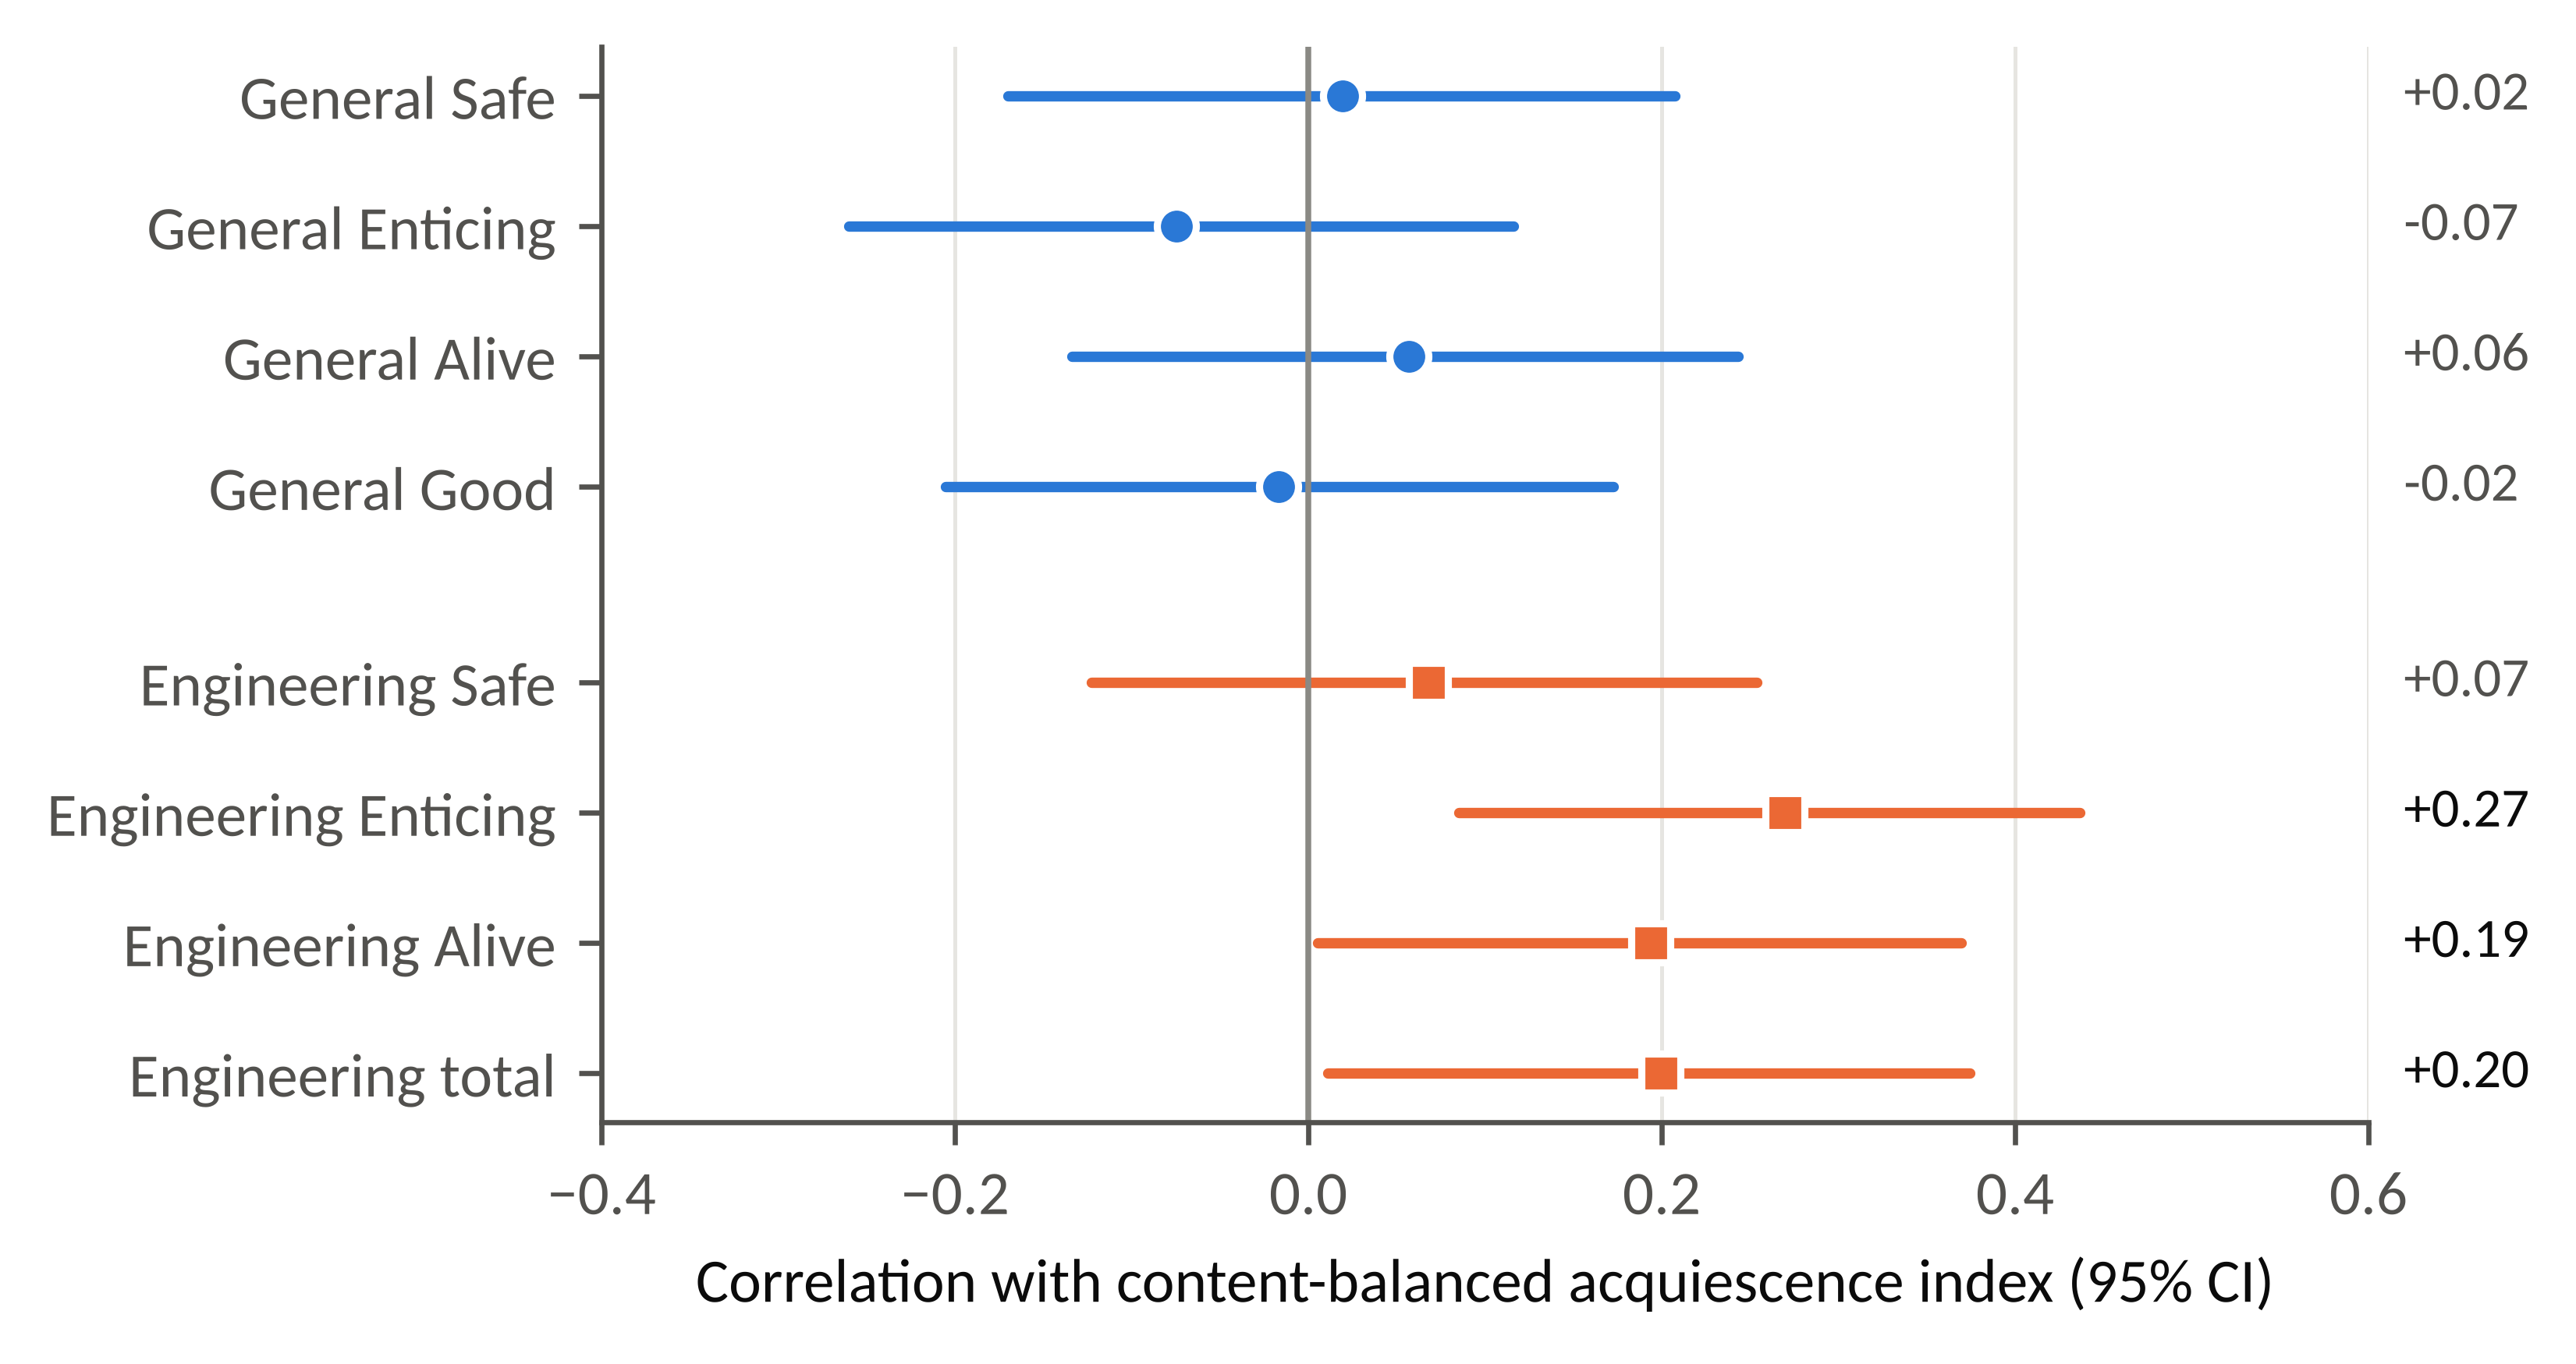
\includegraphics[width=1.0\columnwidth]{fig4_acquiescence.png}
\caption{Correlations (95\% CIs, Fisher $z$) of the content-balanced acquiescence index with general and engineering-specific scales ($N = 108$). Values in black are significant at $p < .05$.}
\label{fig:f4}
\end{figure}

\subsection{Exploratory and Sensitivity Analyses}

Older students reported lower engineering Safe (Spearman $\rho$ = $-$.28, $p$ = .004; $\rho$ = $-$.31, $p$ = .001 after excluding the single 25-year-old). Mean engineering Safe was 3.18–3.19 at ages 17–18, 2.76 at 19 and 2.40 at 20. The association was driven by the career-security items (``stable career'', $\rho$ = $-$.28; ``solid foundation'', $\rho$ = $-$.26; ``secure future'', $\rho$ = $-$.24). It did not survive Holm correction across the 16 exploratory demographic tests (adjusted $p$ = .059), and age was unrelated to any general primal. Sex differences were small and non-significant after correction; with only 11 female respondents, they are not interpreted. Excluding the six long-string responders ($n$ = 102) left the substantive conclusions unchanged (Supplementary Table~\ref{tab:s3}). For example, the engineering-versus-general Safe difference became $d_{\mathrm{z}}$ = 0.78, and parallel analysis still retained two EPB-18 factors.

\section{Discussion}

Four findings stand out. Students saw the world as markedly less safe than reference samples, chiefly because they saw it as competitive and deteriorating; they nevertheless saw engineering as considerably safer, a premium confined to Safe; domain beliefs were only modestly coupled to general primals; and measurement of both kinds of belief was shaped by item keying.

\subsection{A Cut-Throat World}

The low Safe scores are the most striking descriptive result. Students' Safe mean fell about one standard deviation below the reference value, and the item-level pattern was informative: the largest deviations concerned cooperation (``cut-throat and competitive''), regeneration (``getting worse'') and goodness, rather than physical danger or harmlessness. In the vocabulary of Duckitt \emph{et al.}~\cite{duckitt2002}, these students appear to perceive a competitive jungle more than a dangerous world. This interpretation fits the context: for students who have passed through ranked entrance examinations, describing the world as competitive may be closer to accurate reporting than to pessimism~\cite{pienyu2024,subramanian2019}. It also explains a psychometric finding. The ``cut-throat'' item had almost no loading on Safe in this sample, which suggests that, when competition is the norm, perceiving competition does not imply perceiving danger. Whether this reflects a culturally specific meaning of the item or a feature of the educational context cannot be resolved with these data.

Two caveats limit the comparison. First, the reference sample was a general adult online sample recruited through a US-based website, and Clifton and Yaden~\cite{cliftonyaden2021} reported that age correlates positively with Safe ($r$ = .34 for PI-18 Safe in their Study 4). Part of the gap may therefore be developmental rather than cultural or contextual. Second, measurement invariance was not tested, and the keying effects documented here suggest that it may not hold. The comparison is best treated as a benchmark: it shows that these students' Safe scores are low by the instrument's own standards, not that Indian engineering students are less trusting than Americans.

\subsection{A Safe Harbour: Three Candidate Explanations}

The central finding is that, within the same individuals, engineering was rated as considerably safer than the world, whereas it was rated as only marginally more enticing or purposeful. The selectivity of this effect argues against several simple explanations. A general halo around one's own field would elevate all three primals, and the Enticing and Alive differences were negligible. Acquiescence would elevate positively keyed scales, but the Safe difference persisted in the keying-matched comparison, and engineering Safe was the one engineering subscale that was unrelated to the acquiescence index. The safety premium therefore appears to be a genuine feature of how these students view their programmes and is the study's most robust finding.

Why engineering should feel safe in an unsafe world is a separate question, and three explanations are compatible with the data. They are offered as propositions for future testing, not conclusions.

The first is \emph{compensatory control}. When the world is perceived as threatening or uncontrollable, people strengthen their commitment to external systems that promise order~\cite{kay2008,landau2015}. A structured degree programme leading to a recognised profession is such a system. On this account, students do not merely tolerate a dangerous world while studying engineering; they rely on engineering partly \emph{because} the world seems dangerous. The account receives some support from the person-level pattern—most students who leaned towards seeing the world as dangerous nonetheless saw engineering as safe—but it does not straightforwardly predict the positive correlation ($r$ = .30) between general and engineering Safe. A full compensatory account would require that experimentally increasing perceived threat raises engineering Safe, a prediction that can be tested.

The second is \emph{effort justification}. Students who have invested years of preparation, and whose families have often invested heavily too, have strong reasons to view the outcome as secure~\cite{aronson1959}. This account fits the specificity of the effect, because security is the outcome most explicitly promised by the effort, whereas fascination and purpose are not. It also suggests that the premium should be largest at entry and should erode as students encounter the realities of the programme and the labour market.

The third is \emph{realistic relative appraisal}. Engineering may simply be safer than many alternatives available to these students, and students may recognise this. However, evidence of skills gaps and uncertain graduate employment~\cite{blom2011,loyalka2021} suggests that the security of an engineering degree is far from guaranteed, so this account probably cannot explain the full size of the premium.

The exploratory age pattern is relevant to choosing among these explanations. Engineering Safe was highest among 17- and 18-year-olds and lower among 20-year-olds, and the decline was carried by the career-security items, while general Safe showed no age trend. This is the pattern predicted by effort justification followed by reality testing. However, the association did not survive correction for multiple testing, age is only a proxy for year of study, and the data are cross-sectional, so the pattern should be regarded as a hypothesis for longitudinal work. If it replicates, it would identify the middle years of the degree as the period when students' belief in the security of their chosen path is most vulnerable.

\subsection{Domain Beliefs Are Not Simply General Primals Applied}

General primals explained between 12\% and 22\% of the variance in engineering-specific beliefs, and even disattenuated matched correlations were around .40. This is more consistent with the differentiation account than with strong generalisation: knowing how a student sees the world reveals only a modest amount about how they see their discipline. This does not contradict the view of primals as lenses~\cite{clifton2019}, because a lens can colour perception without determining it, but it does indicate that domain beliefs carry substantial independent information. This is encouraging for educators: beliefs about the world are stable~\cite{ludwig2023}, whereas beliefs about a programme are shaped by the programme.

The structure of the engineering-specific items is also theoretically informative. In the general PI-18, Enticing and Alive were only moderately related (latent $r$ = .36), as in the original validation. Within engineering, they were nearly indistinguishable ($r$ = .79), and the items that cross-loaded were those linking fascination with purpose (``full of potential and discovery''; ``important for solving real-world problems''). One interpretation is that, within a vocation, finding the work interesting and finding it meaningful tend to merge, consistent with research showing that purpose for learning sustains engagement with demanding tasks~\cite{yeager2014}. An equally plausible interpretation is that the new items did not separate the two constructs sharply enough. Only a measure with clearer item content can distinguish these possibilities. Security, by contrast, was distinct—and it is the primal that showed the domain premium.

\subsection{Measurement Implications}

Two methodological conclusions follow. First, in this sample the reverse-keyed PI-18 items formed a method factor that markedly improved model fit and was strongest for the Enticing items ``boring'' and ``dull''. This mirrors Bhatnagar and Singh's~\cite{bhatnagar2024} finding of a factor combining the same reverse-keyed items in Indian adults and suggests that their failure to reproduce the three-factor structure was at least partly due to keying effects rather than a different structure of beliefs. One in four students placed ``the world is pretty safe'' and ``the world is dangerous'' on the same side of the scale. This may reflect acquiescence~\cite{smith2004}, lapses in attention, or a dialectical acceptance that the world can be both~\cite{spencer2010}. The current data cannot distinguish among these. Researchers using the PI-18 in India should therefore model keying explicitly, report keying-matched results alongside full-scale scores and include the attention-check item recommended by the instrument's developers.

Second, positively keyed domain instruments can produce misleading positivity. Here, acquiescence accounted for an additional 4\%–8\% of the variance in engineering Enticing and Alive scores, and the EPB-18 total was dominated by a single general factor. A future engineering-specific primal measure should include reverse-keyed items in every subscale, separate career security from in-course coping (the effort-and-perseverance item behaved more like self-efficacy than safety) and write Enticing and Alive items that avoid blending interest with purpose. The present items are a starting point, not a validated scale.

\subsection{Implications for Engineering Education}

Three implications follow, framed with the caution appropriate to cross-sectional data. First, many students enter engineering with a competitive-jungle view of the world. Collaborative learning structures and assessment designs that reward cooperation may therefore do more than build teamwork skills: they may offer direct counter-evidence to the belief that the world is cut-throat. Second, students' sense that engineering is safe appears to be a resource, but potentially a fragile one if it depends on promises that the labour market cannot always keep. Career guidance that is honest about uncertainty while building concrete employability may help students maintain realistic rather than brittle confidence, particularly around the middle of the degree. Third, students' interest in engineering was high (84.3\% above the midpoint on engineering Enticing), but their sense of purpose was lower (63.0\%), and the two were intertwined. Making explicit links between coursework and the problems engineering solves may strengthen both.

\subsection{Limitations}

The study has several important limitations. The sample was a convenience sample of 108 students, overwhelmingly male and young, and eligibility as an engineering student was not independently verified. Institution, discipline and year of study were not recorded, so the findings cannot be generalised to Indian engineering students as a population, and possible clustering within institutions could not be modelled. The sample was adequate for the main within-person effects but small for CFA. The EPB-18 items were newly written and not pretested, and their structure was only partially supported. The PI-18 was administered in grouped rather than validated order without the attention check, which may have inflated within-subscale correlations. Comparisons with the reference sample confound culture, age, recruitment and administration, and they assume measurement invariance that was not tested. No outcome measures (e.g., well-being, engagement or performance) were collected, so the consequences of the safety premium remain unknown. Finally, the design was cross-sectional, and all interpretive accounts, including the age pattern, require longitudinal or experimental tests.

\subsection{Future Research}

Four studies follow directly: a longitudinal study from entry to graduation, testing whether the safety premium declines as effort justification predicts; an experiment manipulating perceived threat or control, testing the compensatory account; a revised, balanced-keyed domain measure validated across institutions; and studies adding well-being, engagement and persistence, testing whether domain Safe buffers a low general Safe—whether a safe harbour protects students or merely postpones disillusionment.

\section{Conclusion}

Indian engineering undergraduates in this sample described the world as considerably less safe than reference samples, largely because they experienced it as competitive and deteriorating. Yet most rated engineering as safe. This domain safety premium was large, robust to item keying, specific to Safe and only modestly predicted by general primals. The study contributes the first within-person comparison of general and domain-specific primals, evidence from an under-studied population and guidance for measuring primals where keying effects are strong. Whether engineering is a lasting safe harbour or a temporary one is the key question for future research.


\section*{Data Availability}
The de-identified response data ($N$ = 108; state recoded to region, time stamps removed), a codebook and the complete analysis code are publicly available at \url{https://github.com/robotics1106/Primal-World-Beliefs-Engineering}. All statistics reported in the article, except the number of states represented and the data-collection dates, can be reproduced from these files. Deviations from standard PI-18 administration, data handling, item-level results, a sensitivity analysis, the codebook and reproduction instructions are given in the Supplementary Material appended to this paper (Sections~\ref{sec:s1}--\ref{sec:s4}).

\section*{Ethical Considerations}
The survey was anonymous and collected no names, contact details, student identifiers or institutional affiliations; only sex, age and state were recorded as demographic information. In the shared dataset, state is recoded to region and time stamps are removed. The study was conducted independently by the author and was not reviewed by an institutional ethics committee. The form stated that participation was voluntary and anonymous, and submitting it was taken as consent; respondents aged 17 ($n$ = 10) took part under the same procedure, and no parental consent was sought.

\section*{Acknowledgment}
The author thanks the students who completed the survey. An AI assistant (Claude, Anthropic) was used to support statistical re-analysis, figure preparation, literature verification and drafting; the author reviewed all analyses and text and takes full responsibility for the content.

\begin{thebibliography}{99}
\providecommand{\url}[1]{#1}
\bibitem{pienyu2024}
K.~Pienyu, B.~Margaret, and A.~D'Souza, ``Academic stress, perceived parental pressure, and anxiety related to competitive entrance examinations and the general well-being among adolescents: A cross-sectional survey from Karnataka, India,'' \emph{J. Educ. Health Promot.}, vol.~13, no.~1, Art. no.~474, 2024, doi: 10.4103/jehp.jehp\_2094\_23.

\bibitem{subramanian2019}
A.~Subramanian, \emph{The Caste of Merit: Engineering Education in India}. Cambridge, MA, USA: Harvard Univ. Press, 2019.

\bibitem{blom2011}
A.~Blom and H.~Saeki, ``Employability and skill set of newly graduated engineers in India,'' World Bank, Washington, DC, USA, Policy Res. Work. Paper 5640, 2011, doi: 10.1596/1813-9450-5640.

\bibitem{loyalka2021}
P.~Loyalka \emph{et al.}, ``Skill levels and gains in university STEM education in China, India, Russia and the United States,'' \emph{Nat. Hum. Behav.}, vol.~5, no.~7, pp.~892--904, 2021, doi: 10.1038/s41562-021-01062-3.

\bibitem{clifton2019}
J.~D.~W. Clifton \emph{et al.}, ``Primal world beliefs,'' \emph{Psychol. Assess.}, vol.~31, no.~1, pp.~82--99, 2019, doi: 10.1037/pas0000639.

\bibitem{cliftonyaden2021}
J.~D.~W. Clifton and D.~B. Yaden, ``Brief measures of the four highest-order primal world beliefs,'' \emph{Psychol. Assess.}, vol.~33, no.~12, pp.~1267--1273, 2021, doi: 10.1037/pas0001055.

\bibitem{kerry2024}
N.~Kerry, K.~C. White, M.~L. O'Brien, L.~M. Perry, and J.~D.~W. Clifton, ``Despite popular intuition, positive world beliefs poorly reflect several objective indicators of privilege, including wealth, health, sex, and neighborhood safety,'' \emph{J. Pers.}, vol.~92, no.~4, pp.~1129--1142, 2024, doi: 10.1111/jopy.12877.

\bibitem{bhatnagar2024}
S.~Bhatnagar and K.~Singh, ``Assessing the psychometric properties of Brief Primal Inventory (PI-18) in Indian setting,'' \emph{J. Indian Acad. Appl. Psychol.}, vol.~50, no.~1, pp.~306--318, 2024.

\bibitem{cliftonmeindl2022}
J.~D.~W. Clifton and P.~Meindl, ``Parents think---incorrectly---that teaching their children that the world is a bad place is likely best for them,'' \emph{J. Posit. Psychol.}, vol.~17, no.~2, pp.~182--197, 2022, doi: 10.1080/17439760.2021.2016907.

\bibitem{ludwig2023}
V.~U. Ludwig, D.~L. Crone, J.~D.~W. Clifton, R.~W. Rebele, J.~A. Schor, and M.~L. Platt, ``Resilience of primal world beliefs to the initial shock of the COVID-19 pandemic,'' \emph{J. Pers.}, vol.~91, no.~3, pp.~838--855, 2023, doi: 10.1111/jopy.12780.

\bibitem{clifton2020}
J.~D.~W. Clifton, ``Testing if primal world beliefs reflect experiences---or at least some experiences identified ad hoc,'' \emph{Front. Psychol.}, vol.~11, Art. no.~1145, 2020, doi: 10.3389/fpsyg.2020.01145.

\bibitem{janoff1989}
R.~Janoff-Bulman, ``Assumptive worlds and the stress of traumatic events: Applications of the schema construct,'' \emph{Soc. Cogn.}, vol.~7, no.~2, pp.~113--136, 1989, doi: 10.1521/soco.1989.7.2.113.

\bibitem{henrich2010}
J.~Henrich, S.~J. Heine, and A.~Norenzayan, ``The weirdest people in the world?'' \emph{Behav. Brain Sci.}, vol.~33, no.~2--3, pp.~61--83, 2010, doi: 10.1017/S0140525X0999152X.

\bibitem{eccles2020}
J.~S. Eccles and A.~Wigfield, ``From expectancy-value theory to situated expectancy-value theory: A developmental, social cognitive, and sociocultural perspective on motivation,'' \emph{Contemp. Educ. Psychol.}, vol.~61, Art. no.~101859, 2020, doi: 10.1016/j.cedpsych.2020.101859.

\bibitem{hidi2006}
S.~Hidi and K.~A. Renninger, ``The four-phase model of interest development,'' \emph{Educ. Psychol.}, vol.~41, no.~2, pp.~111--127, 2006, doi: 10.1207/s15326985ep4102\_4.

\bibitem{yeager2014}
D.~S. Yeager \emph{et al.}, ``Boring but important: A self-transcendent purpose for learning fosters academic self-regulation,'' \emph{J. Pers. Soc. Psychol.}, vol.~107, no.~4, pp.~559--580, 2014, doi: 10.1037/a0037637.

\bibitem{kay2008}
A.~C. Kay, D.~Gaucher, J.~L. Napier, M.~J. Callan, and K.~Laurin, ``God and the government: Testing a compensatory control mechanism for the support of external systems,'' \emph{J. Pers. Soc. Psychol.}, vol.~95, no.~1, pp.~18--35, 2008, doi: 10.1037/0022-3514.95.1.18.

\bibitem{landau2015}
M.~J. Landau, A.~C. Kay, and J.~A. Whitson, ``Compensatory control and the appeal of a structured world,'' \emph{Psychol. Bull.}, vol.~141, no.~3, pp.~694--722, 2015, doi: 10.1037/a0038703.

\bibitem{aronson1959}
E.~Aronson and J.~Mills, ``The effect of severity of initiation on liking for a group,'' \emph{J. Abnorm. Soc. Psychol.}, vol.~59, no.~2, pp.~177--181, 1959, doi: 10.1037/h0047195.

\bibitem{duckitt2002}
J.~Duckitt, C.~Wagner, I.~du~Plessis, and I.~Birum, ``The psychological bases of ideology and prejudice: Testing a dual process model,'' \emph{J. Pers. Soc. Psychol.}, vol.~83, no.~1, pp.~75--93, 2002, doi: 10.1037/0022-3514.83.1.75.

\bibitem{perry2013}
R.~Perry, C.~G. Sibley, and J.~Duckitt, ``Dangerous and competitive worldviews: A meta-analysis of their associations with social dominance orientation and right-wing authoritarianism,'' \emph{J. Res. Pers.}, vol.~47, no.~1, pp.~116--127, 2013, doi: 10.1016/j.jrp.2012.10.004.

\bibitem{marsh1996}
H.~W. Marsh, ``Positive and negative global self-esteem: A substantively meaningful distinction or artifactors?'' \emph{J. Pers. Soc. Psychol.}, vol.~70, no.~4, pp.~810--819, 1996, doi: 10.1037/0022-3514.70.4.810.

\bibitem{weijters2013}
B.~Weijters, H.~Baumgartner, and N.~Schillewaert, ``Reversed item bias: An integrative model,'' \emph{Psychol. Methods}, vol.~18, no.~3, pp.~320--334, 2013, doi: 10.1037/a0032121.

\bibitem{smith2004}
P.~B. Smith, ``Acquiescent response bias as an aspect of cultural communication style,'' \emph{J. Cross-Cult. Psychol.}, vol.~35, no.~1, pp.~50--61, 2004, doi: 10.1177/0022022103260380.

\bibitem{wong2003}
N.~Wong, A.~Rindfleisch, and J.~E. Burroughs, ``Do reverse-worded items confound measures in cross-cultural consumer research? The case of the Material Values Scale,'' \emph{J. Consum. Res.}, vol.~30, no.~1, pp.~72--91, 2003, doi: 10.1086/374697.

\bibitem{spencer2010}
J.~Spencer-Rodgers, M.~J. Williams, and K.~Peng, ``Cultural differences in expectations of change and tolerance for contradiction: A decade of empirical research,'' \emph{Pers. Soc. Psychol. Rev.}, vol.~14, no.~3, pp.~296--312, 2010, doi: 10.1177/1088868310362982.

\bibitem{podsakoff2003}
P.~M. Podsakoff, S.~B. MacKenzie, J.-Y. Lee, and N.~P. Podsakoff, ``Common method biases in behavioral research: A critical review of the literature and recommended remedies,'' \emph{J. Appl. Psychol.}, vol.~88, no.~5, pp.~879--903, 2003, doi: 10.1037/0021-9010.88.5.879.

\bibitem{vonelm2007}
E.~von~Elm \emph{et al.}, ``The Strengthening the Reporting of Observational Studies in Epidemiology (STROBE) statement: Guidelines for reporting observational studies,'' \emph{Lancet}, vol.~370, no.~9596, pp.~1453--1457, 2007, doi: 10.1016/S0140-6736(07)61602-X.

\bibitem{curran2016}
P.~G. Curran, ``Methods for the detection of carelessly invalid responses in survey data,'' \emph{J. Exp. Soc. Psychol.}, vol.~66, pp.~4--19, 2016, doi: 10.1016/j.jesp.2015.07.006.

\bibitem{meade2012}
A.~W. Meade and S.~B. Craig, ``Identifying careless responses in survey data,'' \emph{Psychol. Methods}, vol.~17, no.~3, pp.~437--455, 2012, doi: 10.1037/a0028085.

\bibitem{mcneish2018}
D.~McNeish, ``Thanks coefficient alpha, we'll take it from here,'' \emph{Psychol. Methods}, vol.~23, no.~3, pp.~412--433, 2018, doi: 10.1037/met0000144.

\bibitem{rhemtulla2012}
M.~Rhemtulla, P.~\'E. Brosseau-Liard, and V.~Savalei, ``When can categorical variables be treated as continuous? A comparison of robust continuous and categorical SEM estimation methods under suboptimal conditions,'' \emph{Psychol. Methods}, vol.~17, no.~3, pp.~354--373, 2012, doi: 10.1037/a0029315.

\bibitem{hu1999}
L.~Hu and P.~M. Bentler, ``Cutoff criteria for fit indexes in covariance structure analysis: Conventional criteria versus new alternatives,'' \emph{Struct. Equ. Model.}, vol.~6, no.~1, pp.~1--55, 1999, doi: 10.1080/10705519909540118.

\bibitem{henseler2015}
J.~Henseler, C.~M. Ringle, and M.~Sarstedt, ``A new criterion for assessing discriminant validity in variance-based structural equation modeling,'' \emph{J. Acad. Mark. Sci.}, vol.~43, no.~1, pp.~115--135, 2015, doi: 10.1007/s11747-014-0403-8.

\bibitem{rodriguez2016}
A.~Rodriguez, S.~P. Reise, and M.~G. Haviland, ``Evaluating bifactor models: Calculating and interpreting statistical indices,'' \emph{Psychol. Methods}, vol.~21, no.~2, pp.~137--150, 2016, doi: 10.1037/met0000045.

\bibitem{horn1965}
J.~L. Horn, ``A rationale and test for the number of factors in factor analysis,'' \emph{Psychometrika}, vol.~30, no.~2, pp.~179--185, 1965, doi: 10.1007/BF02289447.

\bibitem{milfont2010}
T.~L. Milfont and R.~Fischer, ``Testing measurement invariance across groups: Applications in cross-cultural research,'' \emph{Int. J. Psychol. Res.}, vol.~3, no.~1, pp.~111--130, 2010, doi: 10.21500/20112084.857.

\bibitem{lakens2013}
D.~Lakens, ``Calculating and reporting effect sizes to facilitate cumulative science: A practical primer for $t$-tests and ANOVAs,'' \emph{Front. Psychol.}, vol.~4, Art. no.~863, 2013, doi: 10.3389/fpsyg.2013.00863.

\bibitem{igolkina2020}
A.~A. Igolkina and G.~Meshcheryakov, ``semopy: A Python package for structural equation modeling,'' \emph{Struct. Equ. Model.}, vol.~27, no.~6, pp.~952--963, 2020, doi: 10.1080/10705511.2019.1704289.

\end{thebibliography}

\clearpage
\onecolumn
\makeatletter\setlength{\@fptop}{0pt}\makeatother
\setcounter{section}{0}\setcounter{table}{0}
\renewcommand{\thesection}{S\arabic{section}}\renewcommand{\theHsection}{supp.\arabic{section}}
\renewcommand{\thetable}{S\arabic{table}}\renewcommand{\theHtable}{supp.\arabic{table}}
\begin{center}
{\LARGE Supplementary Material}\\[6pt]
{\large A Safe Harbour in a Cut-Throat World? General and Engineering-Specific Primal World Beliefs Among Indian Engineering Undergraduates}\\[4pt]
{\normalsize Ritabrata Chakraborty}
\end{center}
\vspace{6pt}

\noindent This supplementary material accompanies the article above. It reports item-level results, a sensitivity analysis, deviations from standard PI-18 administration, a codebook for the shared data file and instructions for reproducing the analyses.

\section{Deviations From Standard PI-18 Administration}\label{sec:s1}

Three features of data collection differed from the administration instructions for the PI-18~\cite{cliftonyaden2021}. First, the 18 items were grouped by intended primal on the form rather than presented in the validated fixed order. Second, the optional attention-check item (``Please mark this statement 'slightly disagree''') was not included. Third, the form grouped ``In life, there's way more beauty than ugliness'' with the Safe items, although the published key assigns it to Enticing. All analyses in the article use the published scoring key, so the third deviation affects presentation order only. The first two may have inflated within-subscale correlations and reduced the ability to screen inattentive responding; both are acknowledged as limitations in the article.

\section{Data Handling}\label{sec:s2}

The survey form recorded 108 complete, time-stamped responses between 13 and 15 October 2024; all are analysed. Responses had been stored on a $-$5 to +5 metric ($-$5 = strongly disagree, $-$3 = disagree, $-$1 = slightly disagree, 1 = slightly agree, 3 = agree, 5 = strongly agree) and were linearly transformed to the published 0–5 metric, ($x$ + 5) / 2. Reverse-keyed PI-18 items were then rescored as 5 $-$ $x$. No values were missing or out of range. An earlier working spreadsheet contained seven additional rows without time stamps that could not be matched to form submissions; these were not analysed.

\begin{table}[!htbp]
\centering
\renewcommand{\arraystretch}{1.15}
\footnotesize
\setlength{\tabcolsep}{3pt}
\caption{Engineering-Specific Primal Belief Items (EPB-18): Wording, Descriptive Statistics and Exploratory Factor Loadings}
\label{tab:s1}
\begin{tabular}{>{\raggedright\arraybackslash}p{0.75cm}>{\raggedright\arraybackslash}p{7.2cm}ccccccc}
\toprule
Code & Item & $M$ & $SD$ & \% agree & $r$(it) & F1 Safe & F2 Enticing & F3 Alive \\
\midrule
ES1 & I feel confident that my engineering degree will provide a secure future. & 2.82 & 1.41 & 60.2 & .59 & .56 & .10 & .03 \\
ES2 & The engineering environment feels safe and supportive. & 2.56 & 1.42 & 55.6 & .68 & .65 & .14 & $-$.03 \\
ES3 & Most challenges in my engineering coursework can be solved with effort and perseverance. & 3.67 & 1.27 & 88.0 & .55 & .35 & .22 & .22 \\
ES4 & I trust that my education is preparing me for a stable career in engineering. & 2.89 & 1.46 & 65.7 & .72 & .79 & .12 & $-$.06 \\
ES5 & My engineering program offers a solid foundation for a reliable future. & 2.78 & 1.38 & 65.7 & .77 & .86 & $-$.03 & .02 \\
ES6 & The academic structure in my engineering program gives me a sense of security. & 2.52 & 1.53 & 53.7 & .71 & .80 & $-$.14 & .11 \\
EE1 & Engineering offers endless opportunities for innovation and creativity. & 3.49 & 1.51 & 79.6 & .59 & .23 & .51 & .02 \\
EE2 & I find the problems we solve in engineering to be exciting and engaging. & 3.30 & 1.41 & 75.0 & .66 & .12 & .50 & .18 \\
EE3 & There is always something new to explore in the field of engineering. & 4.02 & 1.08 & 91.7 & .70 & $-$.02 & .83 & $-$.04 \\
EE4 & The complexity of engineering makes it fascinating to study and work in. & 3.69 & 1.26 & 84.3 & .82 & .02 & .91 & $-$.04 \\
EE5 & I feel energized by the possibilities that engineering brings to the world. & 3.63 & 1.27 & 82.4 & .73 & $-$.05 & .69 & .22 \\
EE6 & The engineering projects I work on are full of potential and discovery. & 3.09 & 1.23 & 72.2 & .61 & $-$.08 & .19 & .70 \\
EA1 & My engineering studies feel purposeful and meaningful. & 2.73 & 1.37 & 61.1 & .68 & .23 & $-$.02 & .67 \\
EA2 & The projects I work on seem to follow a greater goal. & 2.76 & 1.40 & 60.2 & .75 & .00 & $-$.07 & .91 \\
EA3 & I believe my role as an engineer is important for solving real-world problems. & 3.38 & 1.35 & 75.0 & .69 & $-$.05 & .40 & .51 \\
EA4 & I often feel like my education is preparing me for a larger purpose. & 2.80 & 1.47 & 63.0 & .81 & .26 & .11 & .55 \\
EA5 & The challenges I face in engineering help me grow in meaningful ways. & 3.38 & 1.28 & 82.4 & .62 & .22 & .46 & .17 \\
EA6 & The work I do in engineering feels connected to something bigger than myself. & 2.71 & 1.59 & 61.1 & .70 & .23 & .23 & .40 \\
\bottomrule
\end{tabular}

\vspace{3pt}\parbox{\textwidth}{\scriptsize \emph{Note.} $N$ = 108. Items were answered on a six-point scale (strongly disagree to strongly agree) and scored 0–5. \% agree = percentage choosing slightly agree, agree or strongly agree. $r$(it) = corrected item–rest correlation within the intended subscale. Loadings are pattern coefficients from minimum-residual EFA with oblimin rotation (three factors); $| \lambda |$ $\ge$ .40 is the conventional salience threshold. Factor correlations: F1–F2 = .36, F1–F3 = .60, F2–F3 = .60. Item codes: ES = Safe, EE = Enticing, EA = Alive.}
\end{table}

\begin{table}[!htbp]
\centering
\renewcommand{\arraystretch}{1.15}
\footnotesize
\setlength{\tabcolsep}{2.6pt}
\caption{PI-18 Items: Descriptive Statistics, Comparison With Reference Means, and Factor Loadings}
\label{tab:s2}
\begin{tabular}{>{\raggedright\arraybackslash}p{5.0cm}ccccccccccc}
\toprule
Item & $M$ & $SD$ & \% agree & Ref. $M$ & $d$ & $p$ (Holm) & EFA Safe & EFA Ent. & EFA Alive & CFA $\lambda$ & $\lambda$ method \\
\midrule
\multicolumn{12}{l}{\emph{Safe}} \\
\hspace{0.8em}World is pretty safe & 1.97 & 1.36 & 31.5 & 2.89 & $-$0.69 & < .001 & .68 & $-$.08 & .10 & .57 & — \\
\hspace{0.8em}World is dangerous (R) & 2.13 & 1.33 & 68.5 & 2.72 & $-$0.45 & < .001 & .40 & .22 & $-$.15 & .47 & .30 \\
\hspace{0.8em}World is cut-throat, competitive (R) & 1.37 & 1.20 & 86.1 & 2.48 & $-$0.90 & < .001 & .05 & .23 & $-$.18 & .14 & .28 \\
\hspace{0.8em}Things tend to get worse (R) & 2.12 & 1.25 & 60.2 & 3.13 & $-$0.82 & < .001 & .10 & .38 & $-$.12 & .29 & .34 \\
\hspace{0.8em}Most things are good & 2.35 & 1.25 & 46.3 & 3.43 & $-$0.92 & < .001 & .65 & .17 & .02 & .75 & — \\
\hspace{0.8em}Most things harmless, totally safe & 2.29 & 1.36 & 40.7 & 2.65 & $-$0.28 & .03 & .75 & $-$.01 & $-$.01 & .75 & — \\
\multicolumn{12}{l}{\emph{Enticing}} \\
\hspace{0.8em}More beauty than ugliness & 3.21 & 1.39 & 75.0 & 3.84 & $-$0.50 & < .001 & .25 & .41 & .18 & .54 & — \\
\hspace{0.8em}Most things not worth the effort (R) & 3.06 & 1.57 & 35.2 & 3.38 & $-$0.22 & .12 & $-$.15 & .54 & .08 & .54 & .53 \\
\hspace{0.8em}Most things kind of boring (R) & 3.17 & 1.53 & 25.9 & 3.68 & $-$0.38 & .006 & .02 & .80 & $-$.05 & .83 & .71 \\
\hspace{0.8em}World is abundant & 3.81 & 1.16 & 88.0 & 4.13 & $-$0.31 & .02 & .11 & .49 & $-$.00 & .49 & — \\
\hspace{0.8em}World is fascinating & 3.37 & 1.34 & 77.8 & 3.95 & $-$0.49 & < .001 & $-$.13 & .63 & .15 & .57 & — \\
\hspace{0.8em}World is somewhat dull (R) & 3.43 & 1.49 & 25.9 & 3.87 & $-$0.34 & .02 & .07 & .82 & $-$.02 & .87 & .62 \\
\hspace{0.8em}Incredible beauty always around us & 3.28 & 1.50 & 75.0 & 3.96 & $-$0.53 & < .001 & .04 & .50 & .09 & .48 & — \\
\multicolumn{12}{l}{\emph{Alive}} \\
\hspace{0.8em}Events happen to help me & 2.65 & 1.44 & 55.6 & 3.17 & $-$0.38 & .003 & .03 & .05 & .84 & .87 & — \\
\hspace{0.8em}What happens is meant to happen & 2.86 & 1.66 & 58.3 & 2.92 & $-$0.04 & 1.00 & $-$.04 & $-$.09 & .75 & .70 & — \\
\hspace{0.8em}Events lack bigger purpose (R) & 2.51 & 1.41 & 45.4 & 2.95 & $-$0.31 & .01 & $-$.15 & .09 & .46 & .51 & .07 \\
\hspace{0.8em}Universe needs me & 2.43 & 1.67 & 54.6 & 2.96 & $-$0.34 & .010 & $-$.09 & .12 & .75 & .78 & — \\
\hspace{0.8em}Everything happens for a reason & 3.12 & 1.68 & 65.7 & 3.03 & 0.06 & 1.00 & .15 & $-$.06 & .79 & .77 & — \\
\bottomrule
\end{tabular}

\vspace{3pt}\parbox{\textwidth}{\scriptsize \emph{Note.} $N$ = 108. Short item labels are given; full wording is published in Clifton and Yaden~\cite{cliftonyaden2021}. Scores 0–5 after reverse-scoring items marked (R); \% agree refers to the raw (unreversed) statement. Ref. M and the reference SDs used for d are from Study 2 ($N$ = 5,171) of Clifton and Yaden~\cite[online suppl., Table S2]{cliftonyaden2021}; $d$ uses the pooled SD of the two samples. $p$ (Holm) = one-sample t test against the reference mean, Holm-adjusted across 18 items. EFA = pattern coefficients from a three-factor minimum-residual EFA with oblimin rotation (factor correlations .12–.33). CFA $\lambda$ = standardised loading in the three-factor CFA; $\lambda$ method = loading on the orthogonal reverse-keying factor in the extended model.}
\end{table}

\begin{table}[!htbp]
\centering
\renewcommand{\arraystretch}{1.15}
\footnotesize
\setlength{\tabcolsep}{6pt}
\caption{Sensitivity Analysis: Full Sample (N = 108) Versus Sample Excluding Six Long-String Responders (n = 102)}
\label{tab:s3}
\begin{tabular}{>{\raggedright\arraybackslash}p{7.5cm}cc}
\toprule
Quantity & $\alpha$ (full / reduced) & Estimate (full / reduced) \\
\midrule
General Safe (PI-18) & .68 / .69 & 2.04 / 2.01 \\
General Enticing (PI-18) & .82 / .82 & 3.33 / 3.30 \\
General Alive (PI-18) & .85 / .85 & 2.71 / 2.68 \\
General Good (PI-18) & .82 / .81 & 2.71 / 2.68 \\
Engineering Safe (EPB-18) & .87 / .83 & 2.87 / 2.85 \\
Engineering Enticing (EPB-18) & .87 / .82 & 3.54 / 3.56 \\
Engineering Alive (EPB-18) & .89 / .86 & 2.96 / 2.95 \\
Engineering total (EPB-18) & .94 / .91 & 3.12 / 3.12 \\
$d_{\mathrm{z}}$ Engineering $-$ General Safe &  & 0.72 / 0.78 \\
$d_{\mathrm{z}}$ Engineering $-$ General Enticing &  & 0.18 / 0.25 \\
$d_{\mathrm{z}}$ Engineering $-$ General Alive &  & 0.18 / 0.20 \\
$r$ General Safe – Engineering Safe &  & .30 / .29 \\
Parallel analysis: EPB-18 factors retained &  & 2 / 2 \\
EPB-18 first-eigenvalue variance share &  & 48.4\% / 39.5\% \\
\bottomrule
\end{tabular}

\vspace{3pt}\parbox{\textwidth}{\scriptsize \emph{Note.} Long-string responders gave the identical response to 18 consecutive items (spanning the EPB-18 block in all six cases). Four of the six answered every engineering item positively and two answered every engineering item negatively; such uniform answers may be genuine, so exclusion is reported only as a sensitivity check.}
\end{table}

\section{Codebook for pwb\_engineering\_deidentified.csv}\label{sec:s3}

\emph{id} — sequential respondent number (1–108), in order of submission.

\emph{sex} — 1 = male, 0 = female, as coded in the original form export.

\emph{age} — age in years (17–25).

\emph{region} — region of the state or union territory reported by the respondent (North, West, South, East, Central). North: Uttar Pradesh, Rajasthan, Delhi, Haryana, Punjab, Uttarakhand, Himachal Pradesh, Chandigarh. West: Maharashtra, Gujarat. South: Karnataka, Telangana, Andhra Pradesh, Kerala, Tamil Nadu. East: West Bengal, Bihar, Odisha. Central: Chhattisgarh, Madhya Pradesh.

\emph{P\_\ldots{}} — the 18 PI-18 items in raw form ($-$5 to +5; not reverse-scored). Codes: P\_safe, P\_dangerous (R), P\_cutthroat (R), P\_worse (R), P\_good, P\_harmless (Safe); P\_beautyugly, P\_worth (R), P\_boring (R), P\_abundant, P\_fascinating, P\_dull (R), P\_beautyaround (Enticing); P\_helpme, P\_meant, P\_lackpurpose (R), P\_needsme, P\_reason (Alive). Good comprises the Safe and Enticing items plus P\_helpme and P\_needsme.

\emph{ES1–ES6, EE1–EE6, EA1–EA6} — the 18 engineering-specific items (EPB-18) in raw form ($-$5 to +5); wording in Table~\ref{tab:s1}.

\section{Reproducing the Analyses}\label{sec:s4}

The data file and scripts are available at \url{https://github.com/robotics1106/Primal-World-Beliefs-Engineering}. Running \texttt{python analysis.py pwb\_engineering\_deidentified.csv output\_folder} (Python 3.13; pandas, NumPy, SciPy, statsmodels, factor\_analyzer 0.5.1, semopy 2.3.11) writes all statistics to \texttt{results.json}. Bootstrap procedures use a fixed random seed (20241013), so the reported values are reproduced exactly. When \texttt{results.json} is written to the default \texttt{out/} folder beside the scripts, running \texttt{tables.py} and \texttt{figures.py} regenerates the tables and figures. Results obtained from the shared file are identical to those obtained from the original export, apart from the number of states and the time stamps, which were removed.

\end{document}
